
\documentclass{beamer}

\mode<presentation> {

% The Beamer class comes with a number of default slide themes
% which change the colors and layouts of slides. Below this is a list
% of all the themes, uncomment each in turn to see what they look like.

%\usetheme{default}
\usetheme{AnnArbor}
%\usetheme{Antibes}
%\usetheme{Bergen}
%\usetheme{Berkeley}
%\usetheme{Berlin}
%\usetheme{Boadilla}
%\usetheme{CambridgeUS}
%\usetheme{Copenhagen}
%\usetheme{Darmstadt}
%\usetheme{Dresden}
%\usetheme{Frankfurt}
%\usetheme{Goettingen}
%\usetheme{Hannover}
%usetheme{Ilmenau}
%\usetheme{JuanLesPins}
%\usetheme{Luebeck}
%\usetheme{Madrid}
%\usetheme{Malmoe}
%\usetheme{Marburg}
%\usetheme{Montpellier}
%\usetheme{PaloAlto}
%\usetheme{Pittsburgh}
%\usetheme{Rochester}
%\usetheme{Singapore}
%\usetheme{Szeged}
%\usetheme{Warsaw}

% As well as themes, the Beamer class has a number of color themes
% for any slide theme. Uncomment each of these in turn to see how it
% changes the colors of your current slide theme.

%\usecolortheme{albatross}
\usecolortheme{beaver}
%\usecolortheme{beetle}
%\usecolortheme{crane}
%\usecolortheme{dolphin}
%\usecolortheme{dove}
%\usecolortheme{fly}
%\usecolortheme{lily}
%\usecolortheme{orchid}
%\usecolortheme{rose}
%\usecolortheme{seagull}
%\usecolortheme{seahorse}
%\usecolortheme{whale}
%\usecolortheme{wolverine}

%\setbeamertemplate{footline} % To remove the footer line in all slides uncomment this line
%\setbeamertemplate{footline}[page number] % To replace the footer line in all slides with a simple slide count uncomment this line

%\setbeamertemplate{navigation symbols}{} % To remove the navigation symbols from the bottom of all slides uncomment this line
}
\usepackage{wrapfig}
\usepackage{eso-pic}
\usepackage{graphicx} % Allows including images
\usepackage{booktabs} % Allows the use of \toprule, \midrule and \bottomrule in tables
\usepackage{multicol}
% \newcommand\AtPagemyUpperLeft[1]{\AtPageLowerLeft{%
% \put(\LenToUnit{0.8\paperwidth},\LenToUnit{0.9\paperheight}){#1}}}
% \AddToShipoutPictureFG{
%   \AtPagemyUpperLeft{{
\includegraphics[width=1.5cm,keepaspectratio]{CSUFlogo.png}}}
% }%
\newcommand\AtPagemyLeft[1]{\AtPageLowerLeft{%
\put(\LenToUnit{0.86\paperwidth},\LenToUnit{0.89\paperheight}){#1}}}
\AddToShipoutPictureFG{
  \AtPagemyLeft{{
\includegraphics[width=1.6cm,keepaspectratio]{LOGO.png}}}
}%

%----------------------------------------------------------------------------------------
%	TITLE PAGE
%----------------------------------------------------------------------------------------

\title{Statistical Modeling in Paleoclimatology}



\author{Quynh Thi Ho} % Your name
\institute[CSUF] % Your institution as it will appear on the bottom of every slide, may be shorthand to save space
{
\includegraphics[height=2cm,width=4cm]{CSUFlogo.png}}


\date[Thesis Defense] {Thesis Defense\\ 
April 18 $^{\text{th}}$, 2018} % Date, can be changed to a custom date
\begin{document}
\begin{frame}
\titlepage % Print the title page as the first slide
\end{frame}

\begin{frame}
\frametitle{Overview} % Table of contents slide, comment this block out to remove it
\tableofcontents % Throughout your presentation, if you choose to use \section{} and \subsection{} commands, these will automatically be printed on this slide as an overview of your presentation
\end{frame}

%----------------------------------------------------------------------------------------
%	PRESENTATION SLIDES
%----------------------------------------------------------------------------------------

%------------------------------------------------
\section{Cross-Disciplinary Collaboration } 

\begin{frame}

\frametitle{Big Picture}

\begin{itemize} 

\item<1-> \textbf{Techniques:} Tree Rings vs. Radio Carbon Dating.

\item<2-> \textbf{Water:} Where, Why, When and How Much.

 %why we choose sand as proxy for wetness and not tree rings, comparing drought over 1,000 years as opposed to 10,000 etc.  %new in the field, need to start somewhere with the directions, where to put money.
\item<3-> \textbf{\emph{Climate Change}} % the ultimate goal is to explain climate change

\end{itemize}

\end{frame}


\subsection{Geologists} % A subsection can be created just before a set of slides with a common theme to further break down your presentation into chunks

\begin{frame}

\only<1>{
\begin{center}

\includegraphics[width=0.5\textwidth]{CSUFlogo.png}
\end{center}
} 

\only<2>{
\begin{itemize} 
\item \textbf{Sample:} Lacustrine sample
	\begin{itemize}
	\item Sand composition
    \item Organic objects
	\end{itemize}
\vspace*{-1.5in}
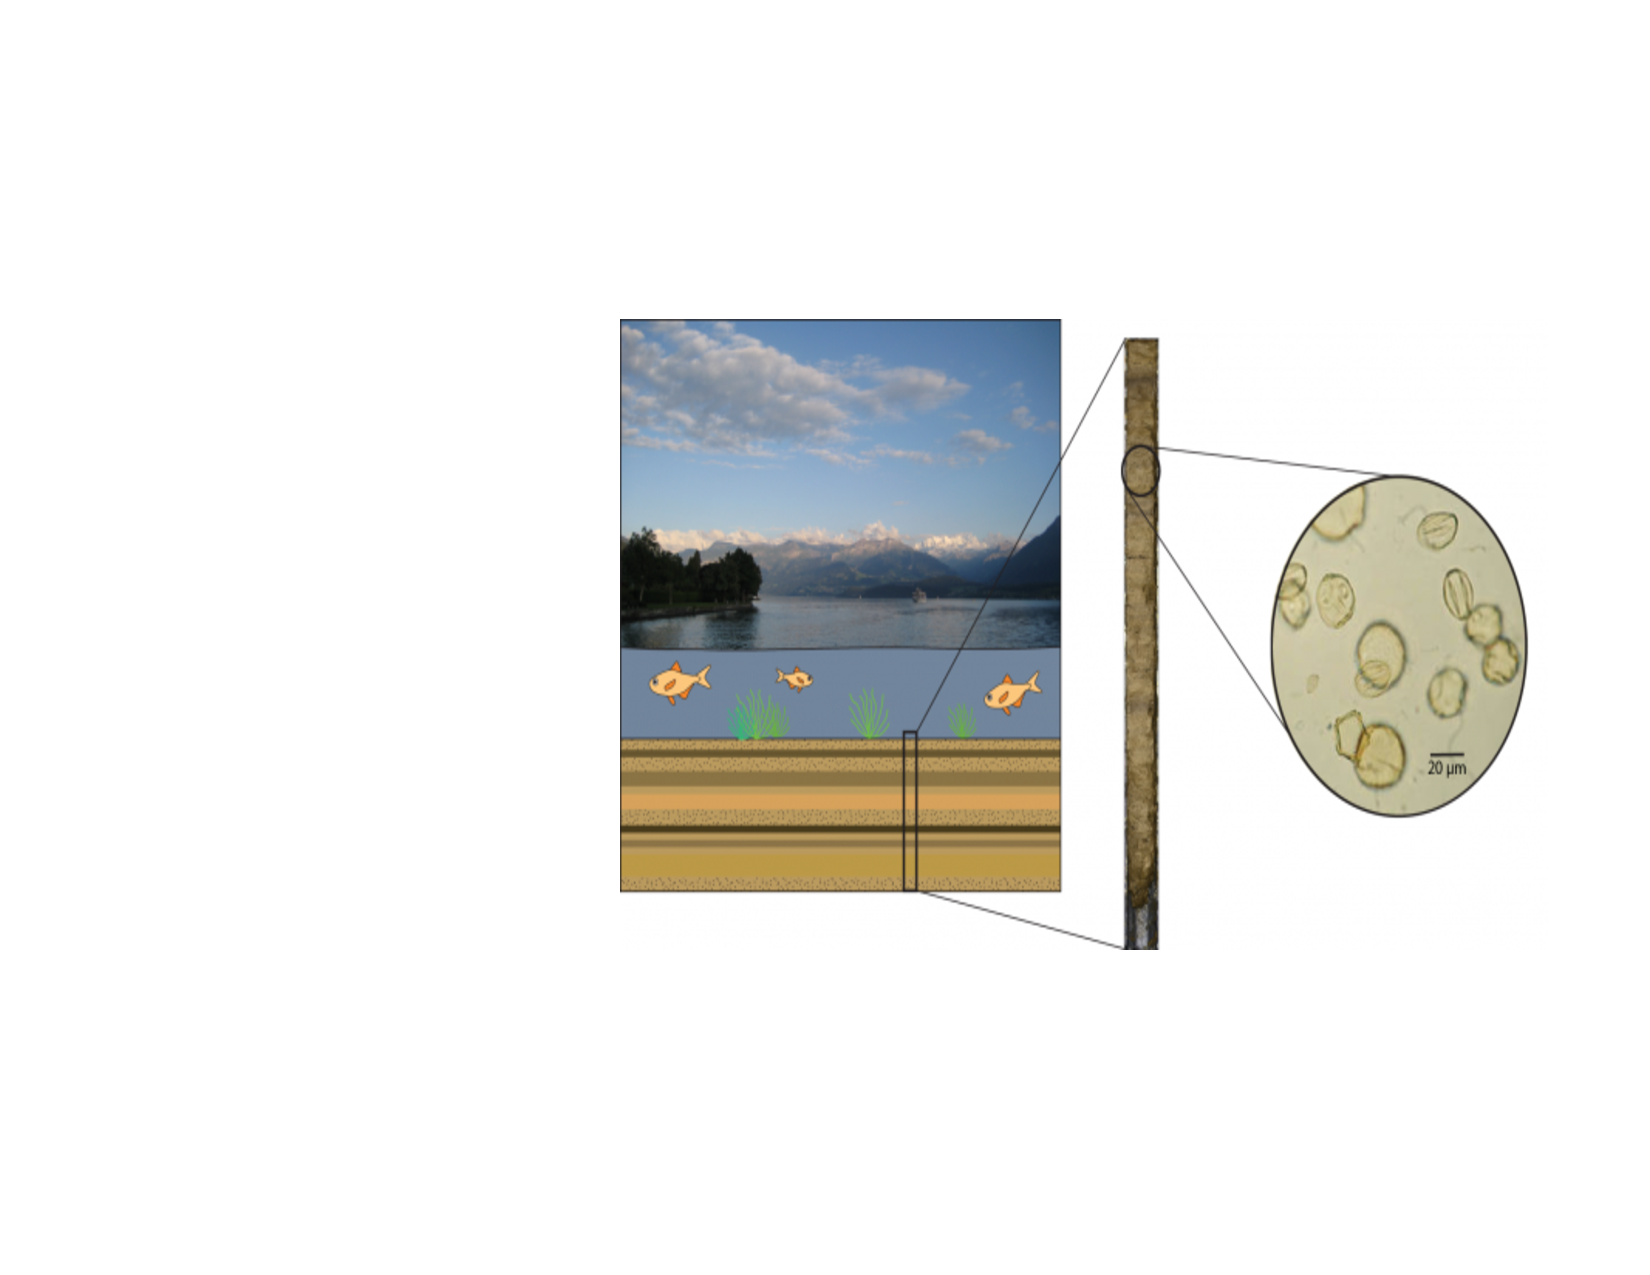
\includegraphics[width=1\textwidth]{cores.pdf}
\vspace*{-1.5in}

\end{itemize}
}
\frametitle{Process of Collecting Data}
%\end{frame}
%\begin{frame}
%\pause

\only<3>{
\vspace{-.3in}
\begin{center}
\hspace*{-.4in}
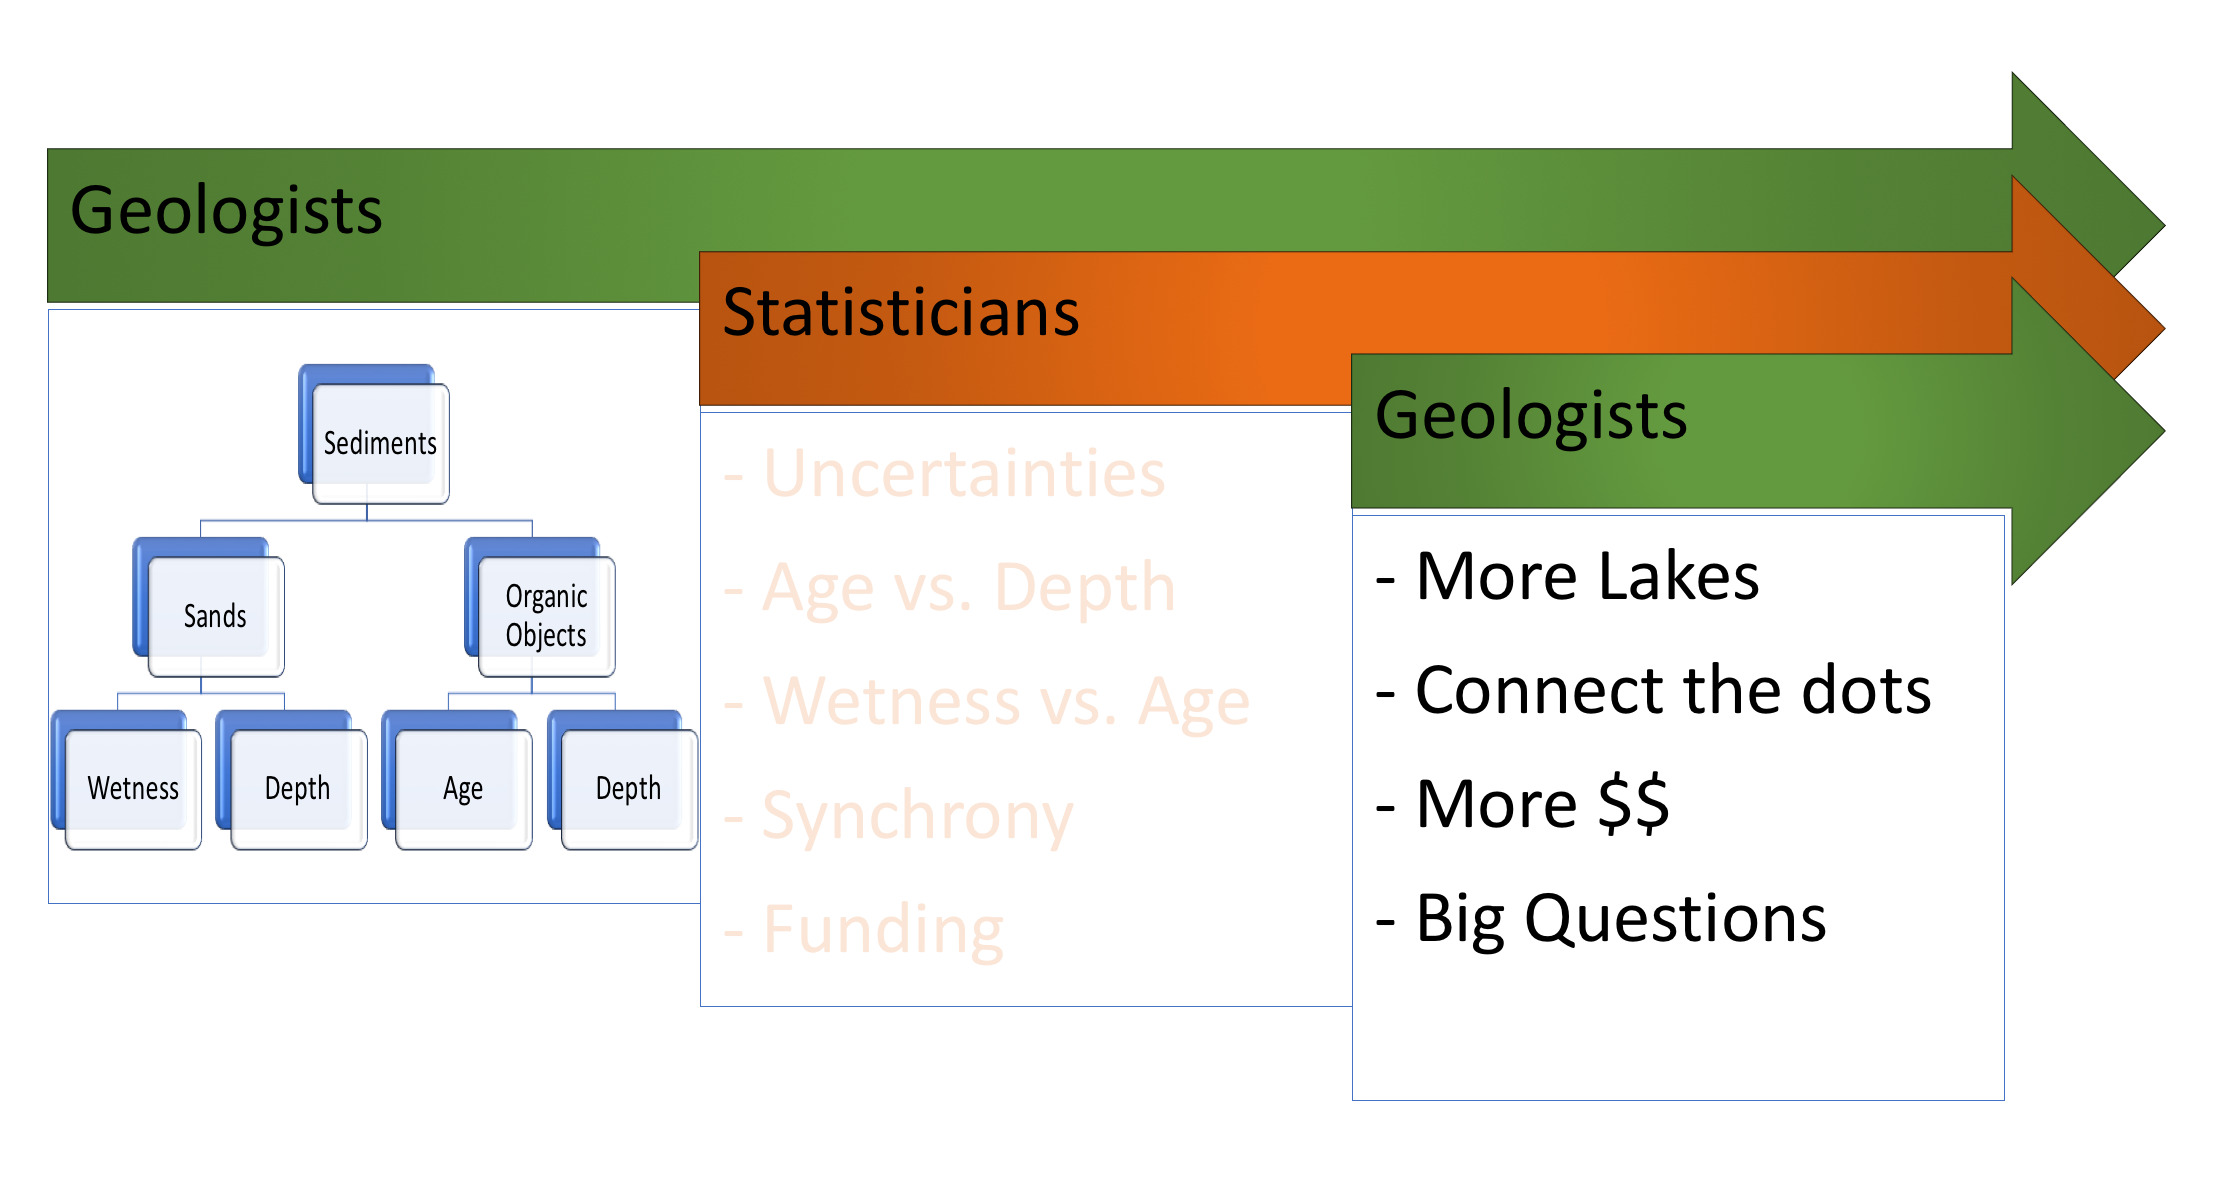
\includegraphics[width=1\textwidth]{page9}
\end{center}
}


\only<4>{
\vspace{-.3in}
\begin{center}
\hspace*{-.4in}
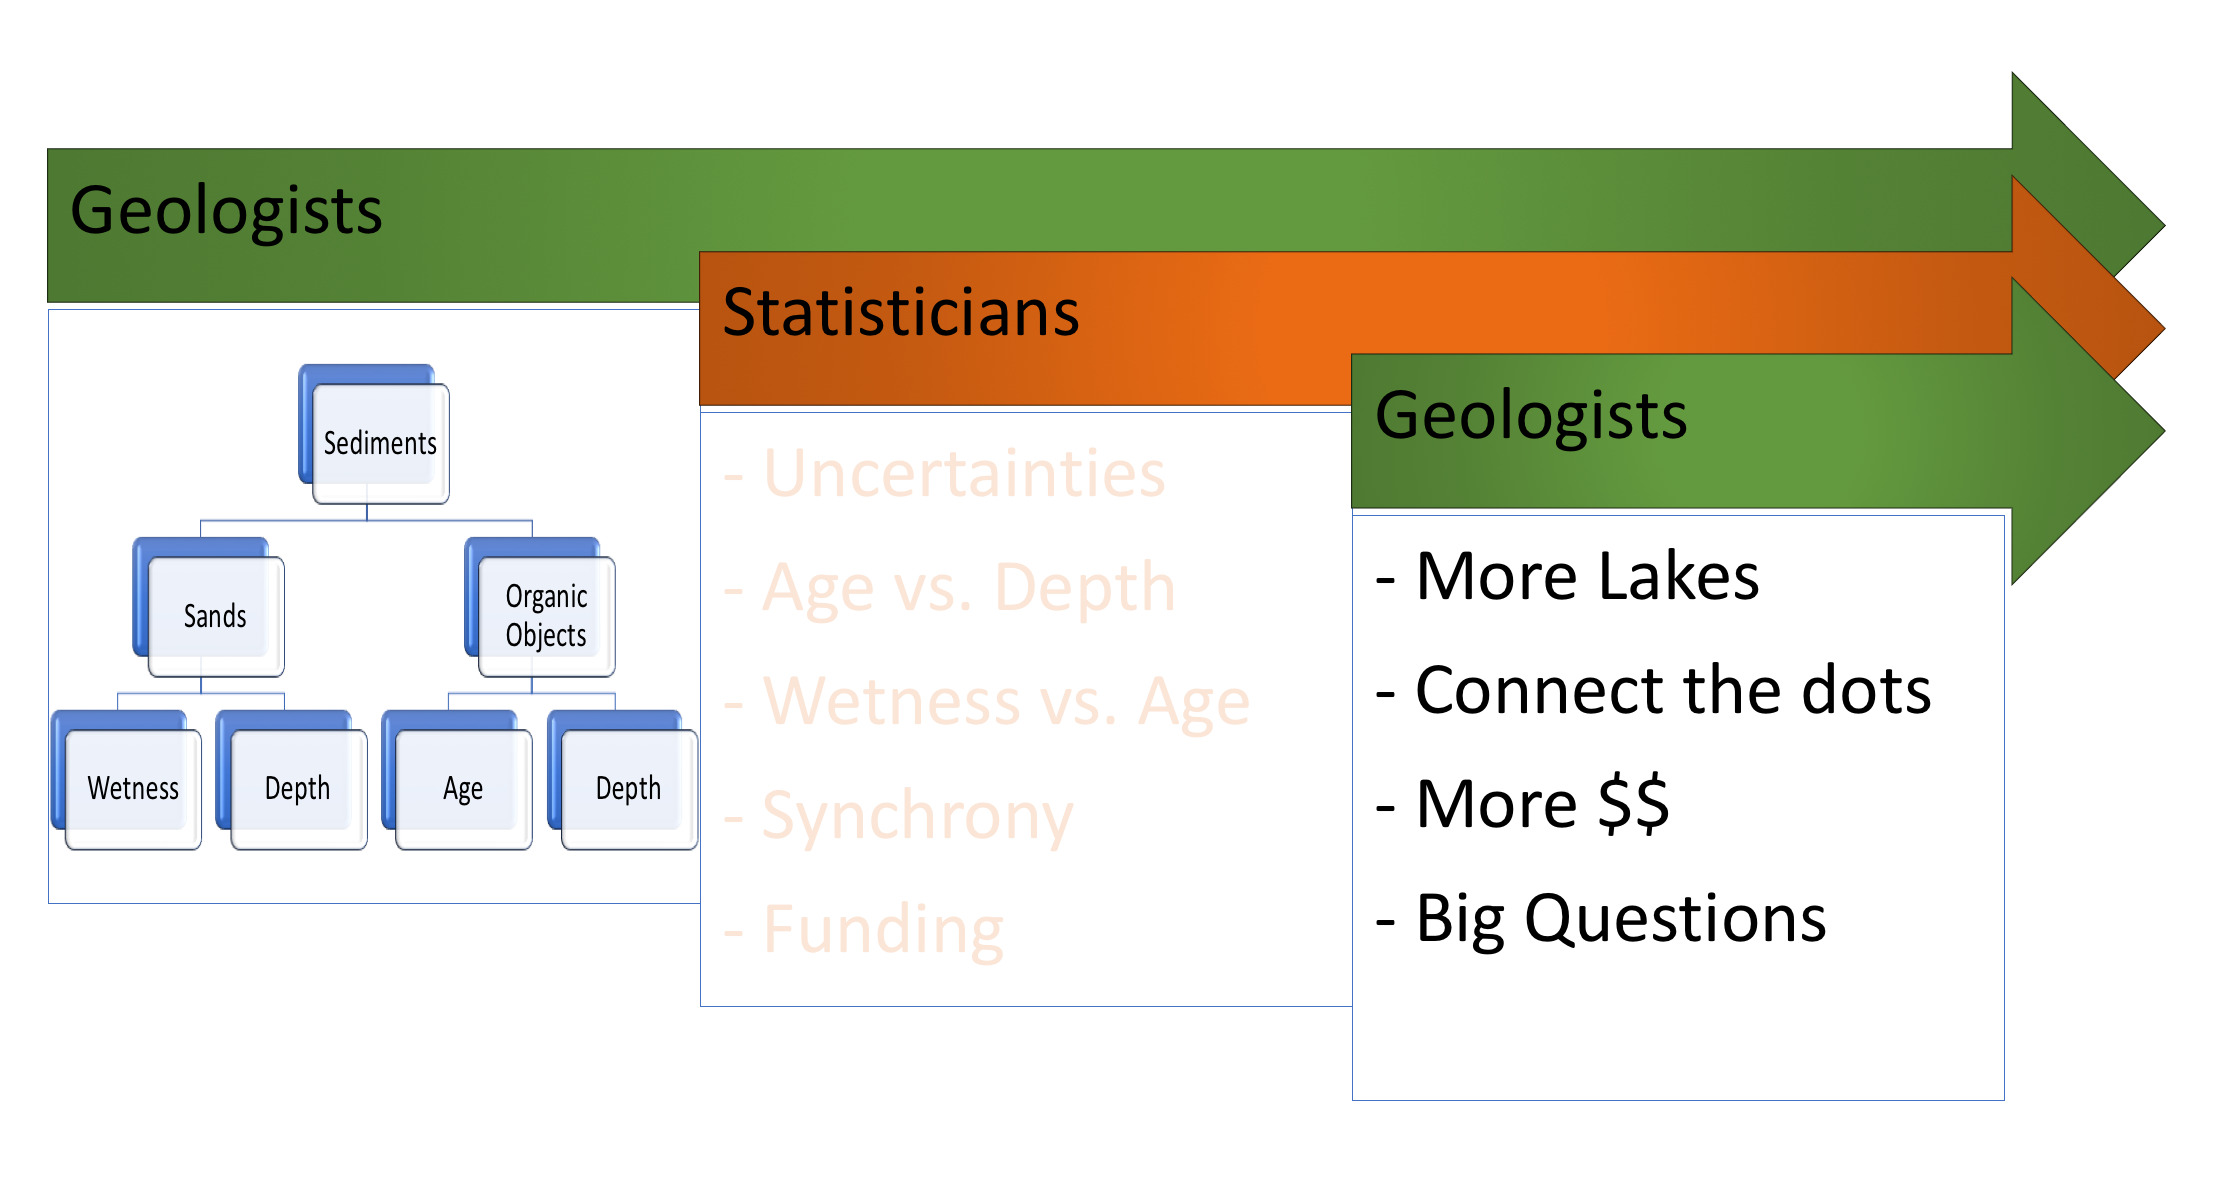
\includegraphics[width=1\textwidth]{page9}
\end{center}
}


\end{frame}

\begin{frame}

\only<1>{
\hspace*{-.2in}
\begin{itemize}
\item \textbf{Data}
	\begin{itemize}
	\item Zaca Lake: $n_{cd} = 20$, \\$n_{\text{ laser}} = 850$
    \item Abbott Lake: $n_{cd} = 5$, \\$n_{\text{ laser}} = 117$
	\end{itemize}
\item Depth: fixed values
\item Wetness: sand composition
\item Age: random variable\\derived from carbon dates 
\end{itemize}
\vspace*{-1.9in}
\hspace*{.3in}
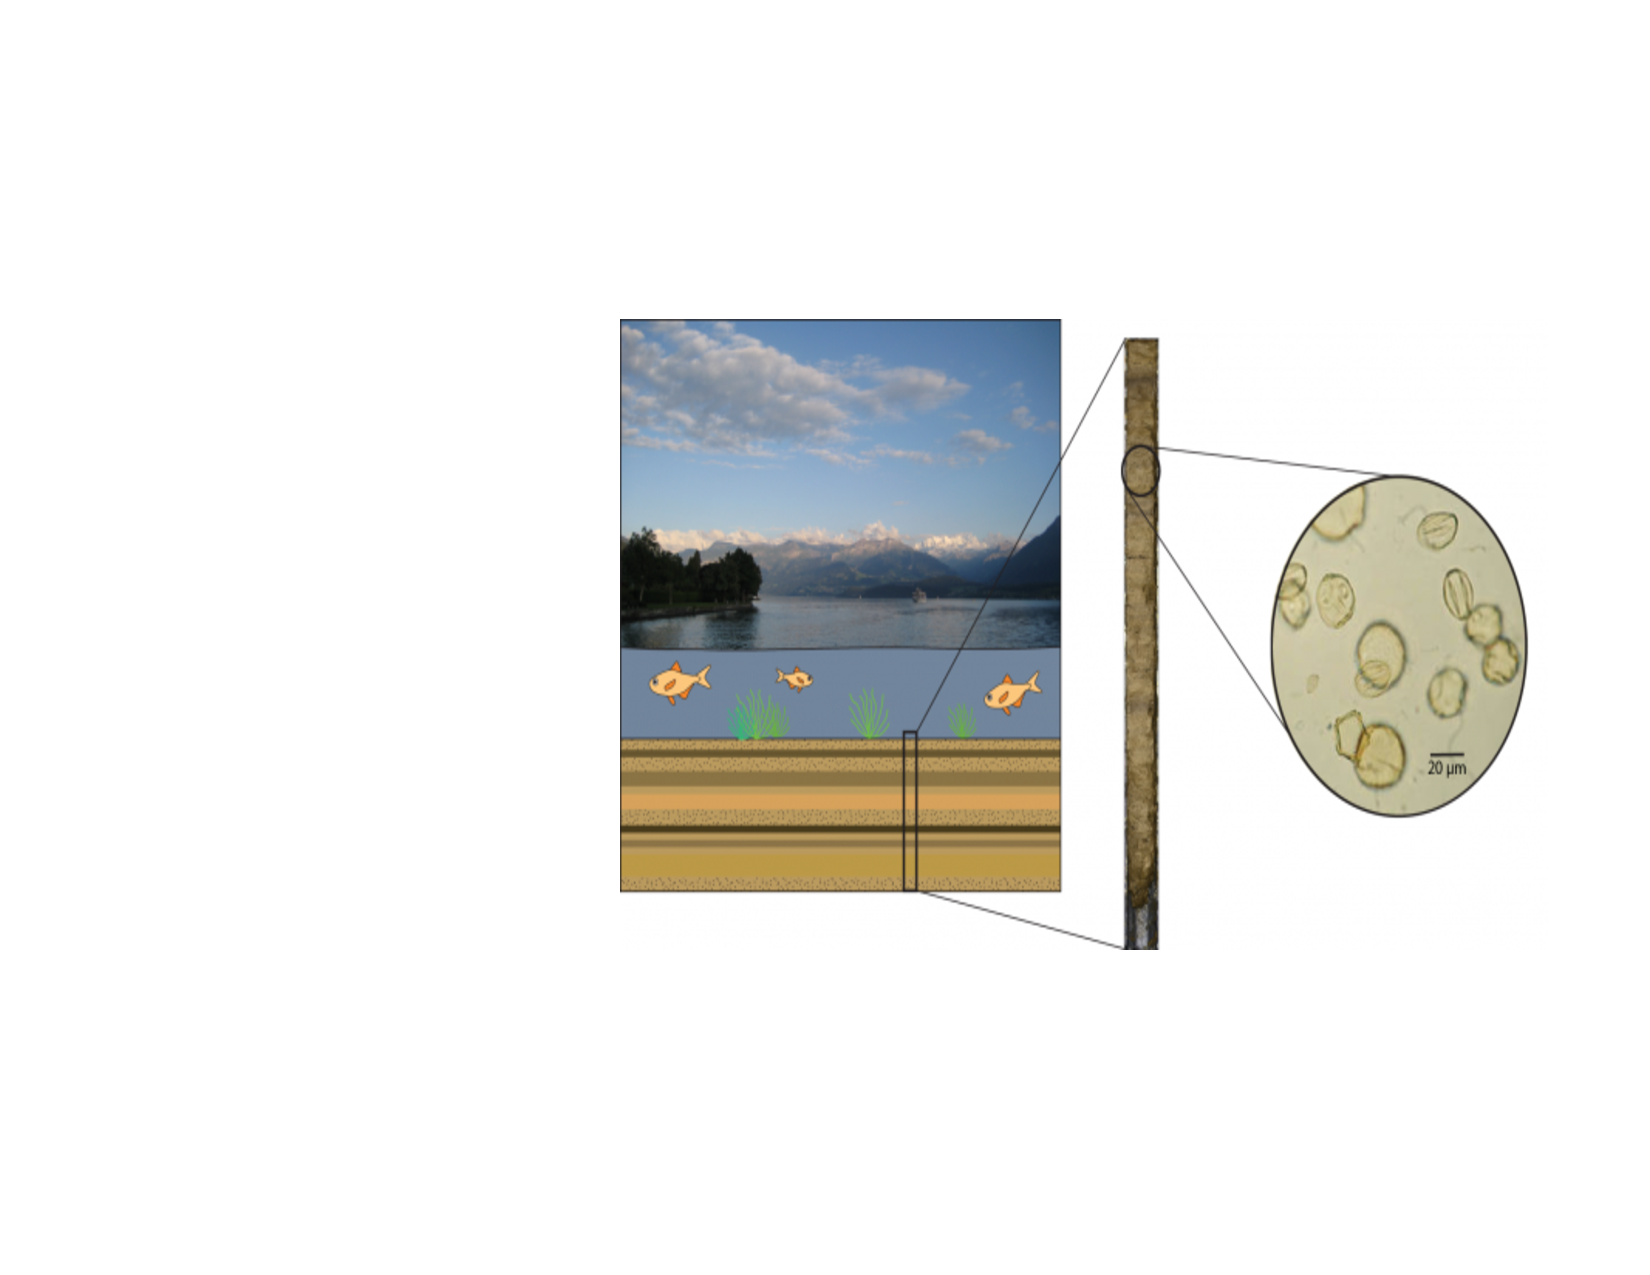
\includegraphics[width=1\textwidth]{cores.pdf}
\vspace*{-0.6in}
}
\frametitle{Data}

\only<2>{
\vspace{-.3in}
\begin{center}
\hspace*{-.3in}
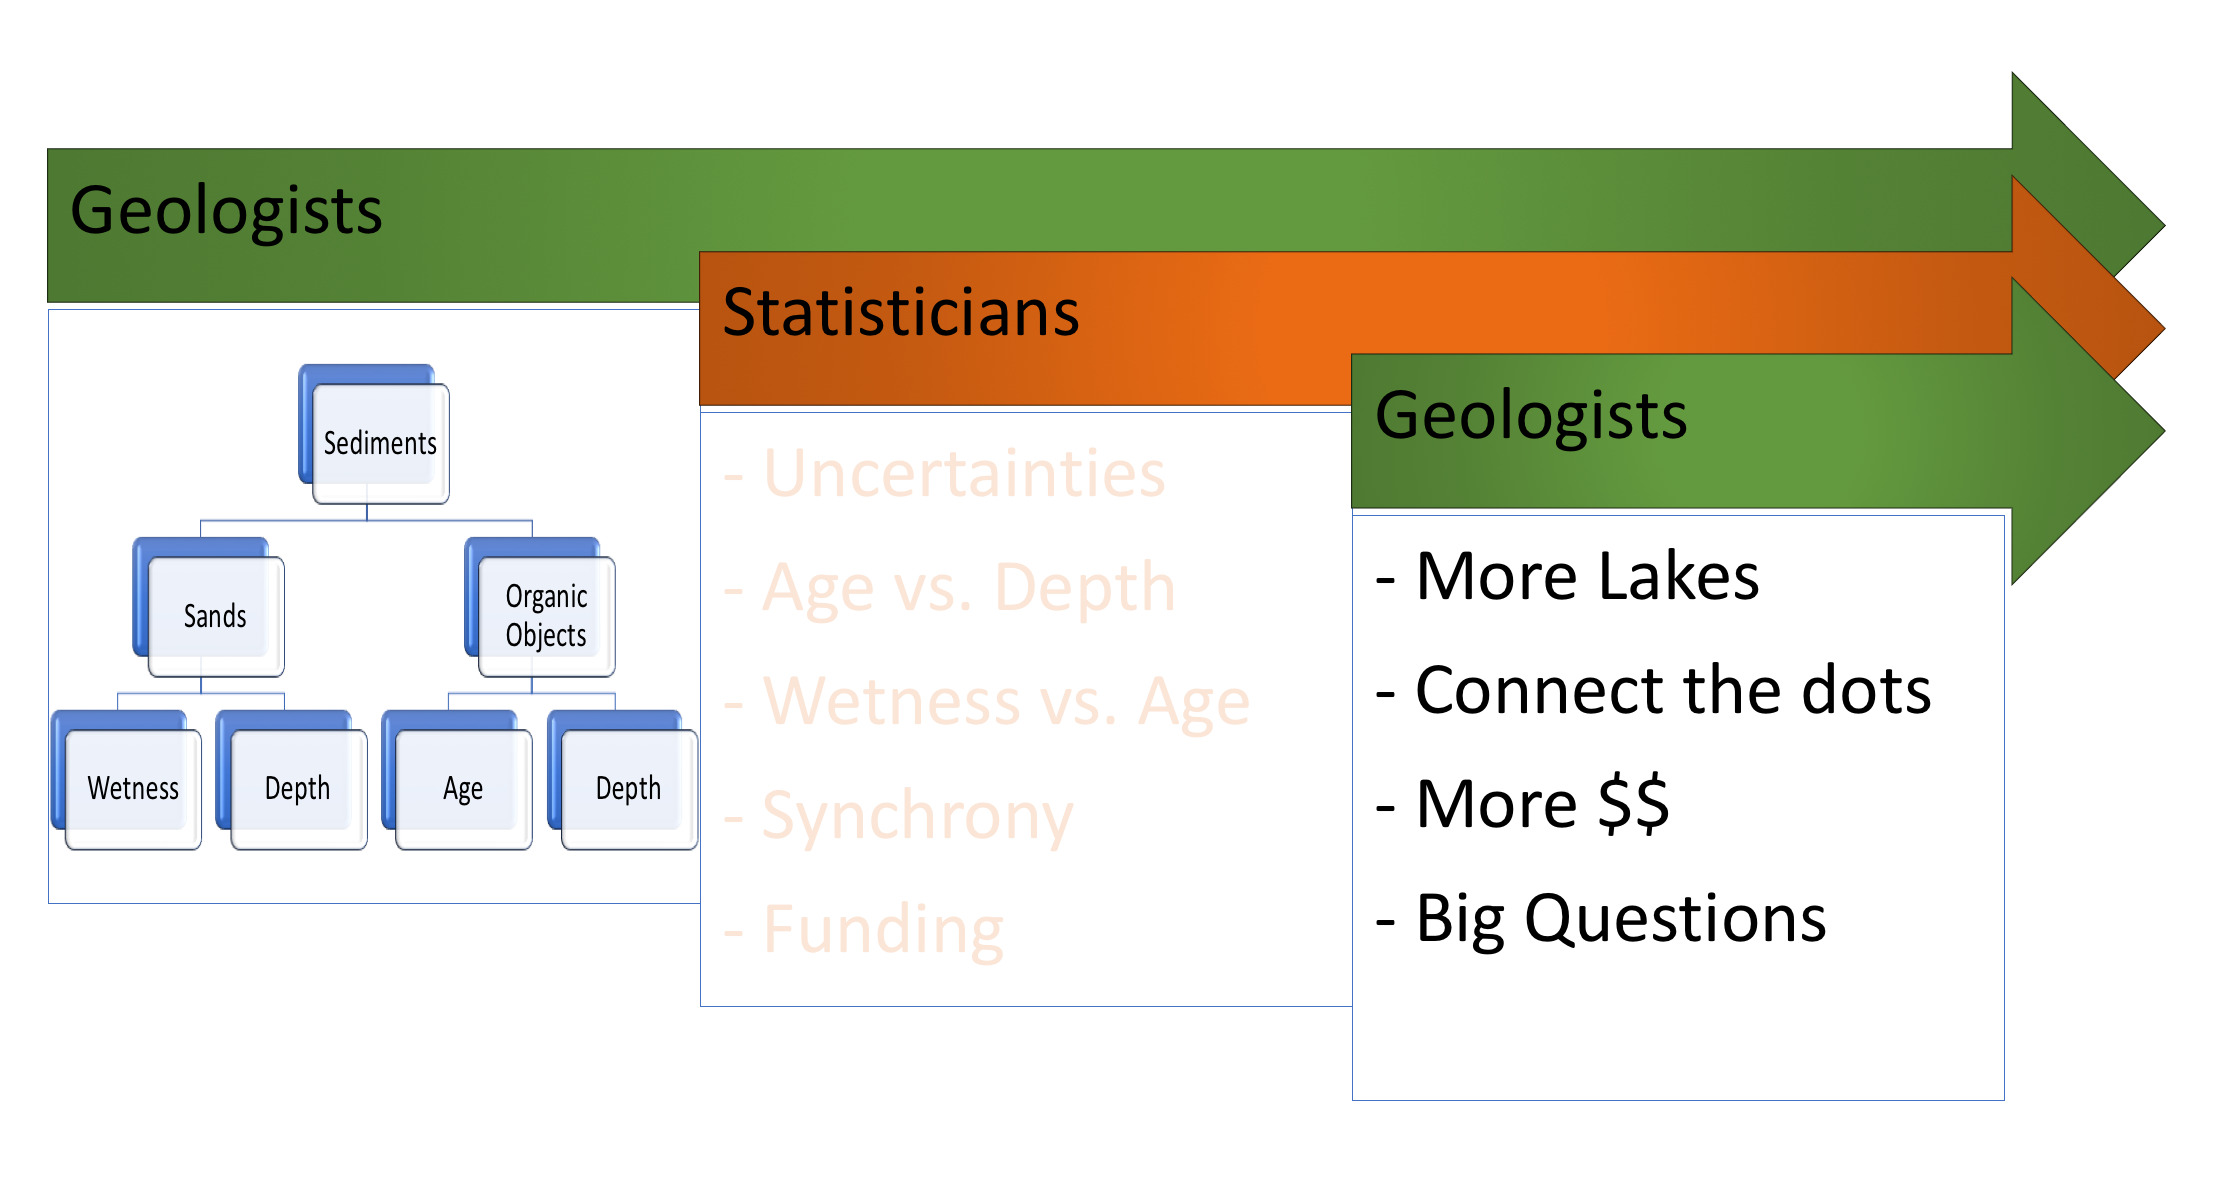
\includegraphics[width=1\textwidth]{page9}
\end{center}
}
\end{frame}


\subsection{Statisticians}
\begin{frame}
\frametitle{Statisticians' Roles}
\begin{itemize}
\item<1-> \textbf{Available Information:} 
    \begin{multicols}{2}	
    	\begin{itemize}
    \item Wetness vs. Depth
    \item Age vs. Depth
	\end{itemize}
    \end{multicols}


\item<2-> \textbf{Ultimate goal}
    \begin{multicols}{2}	
    	\begin{itemize}
    \item Wetness vs. Age
    \item Learn
	\end{itemize}
    \end{multicols}
    \end{itemize}
\end{frame}





\begin{frame}
\frametitle{Process}

\only<1>{
\vspace{-.3in}
\begin{center}
\hspace*{-.3in}
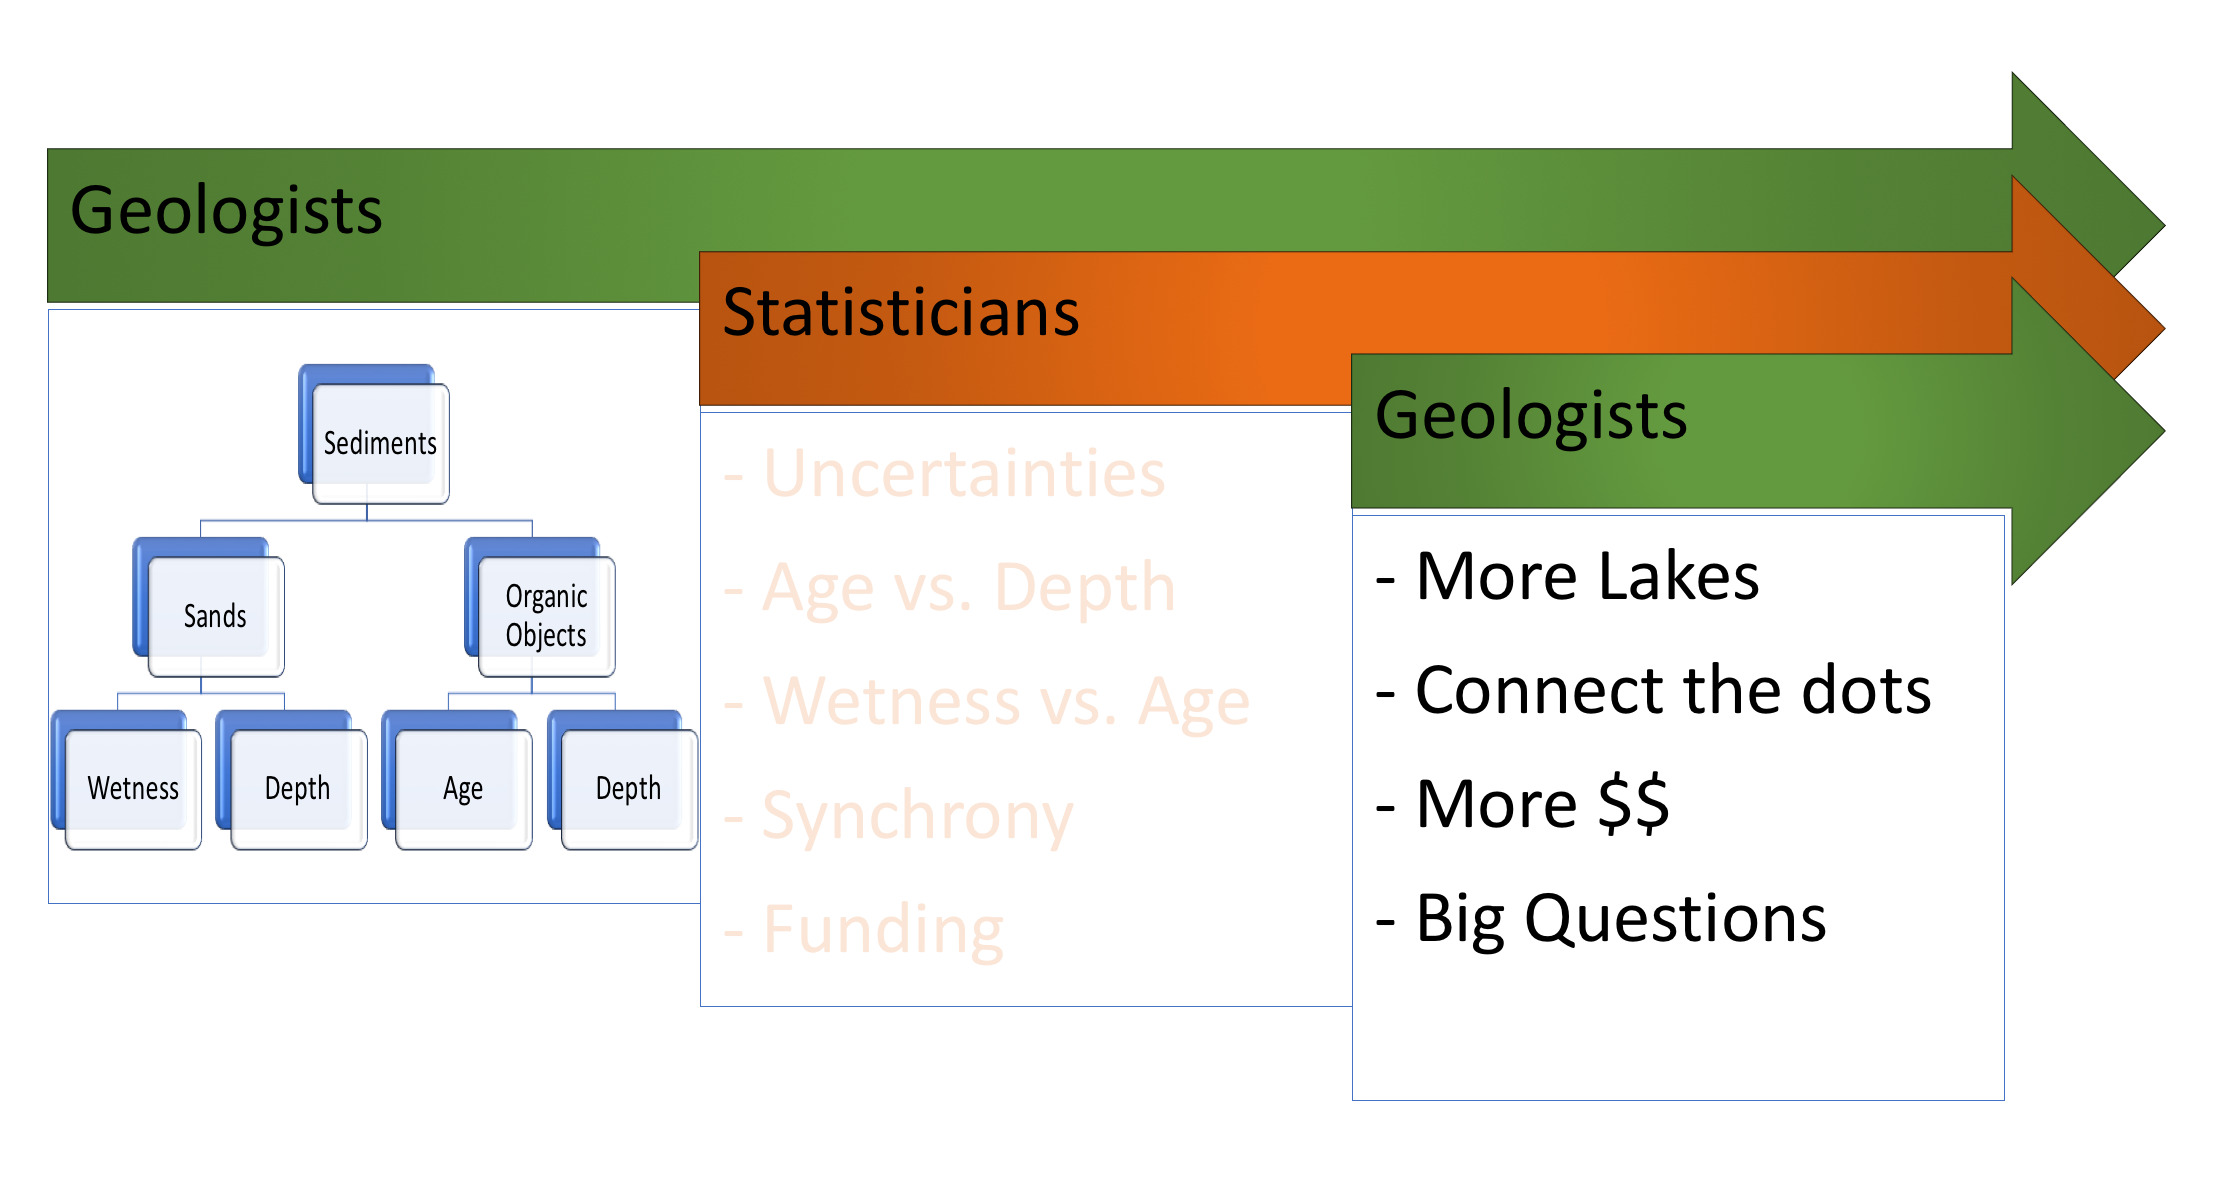
\includegraphics[width=1\textwidth]{page9}
\end{center}
}


\only<2>{
\vspace{-.3in}
\begin{center}
\hspace*{-.3in}
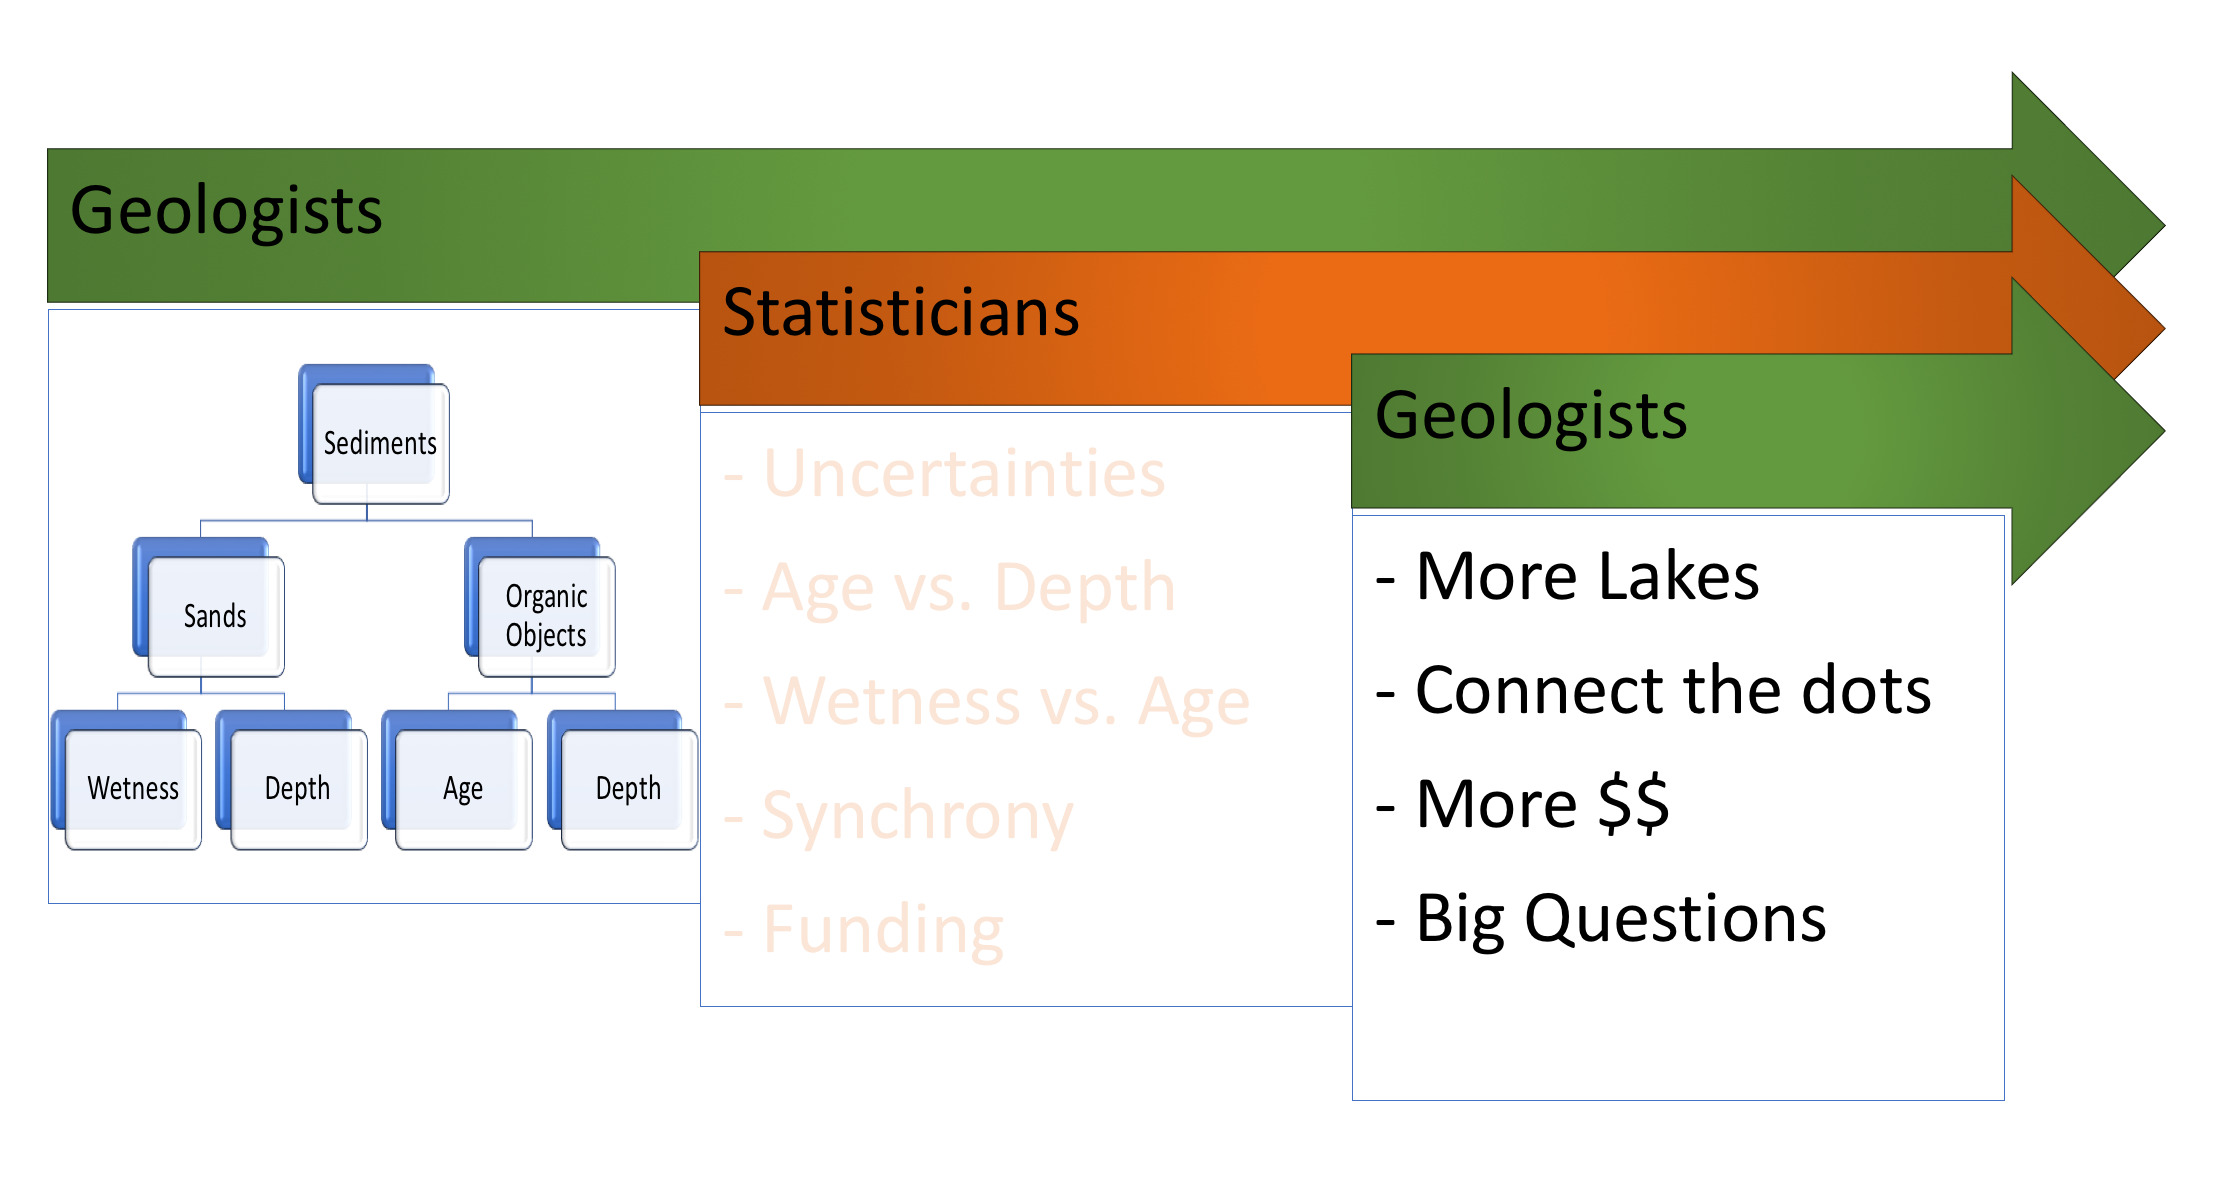
\includegraphics[width=1\textwidth]{page9}
\end{center}
}

\end{frame}





\begin{frame}
\frametitle{Age vs. Depth - BACON}
\only<1>
{\begin{figure}
\hspace*{-.2in}

\includegraphics[width=.5\linewidth]{CSUFlogo.png}

\includegraphics[width=.5\linewidth]{CSUFlogo.png}
\end{figure}}

\only<2>
{\begin{itemize}
	\item<1-> Depth $$ \bf D:=(d_1, d_2, \ldots, d_n)$$
	\item<2-> Restrictions
	\begin{itemize}
		\item Age should be increasing monotonically with depth
		\item Cores may have missing sections
	\end{itemize}
  \end{itemize}
  
}

\only<3>
{\begin{figure}
\hspace*{-.2in}

\includegraphics[width=0.8\linewidth]{CSUFlogo.png}
\end{figure}}

\only<4>
{\begin{figure}
\hspace*{-.2in}

\includegraphics[width=0.8\linewidth]{CSUFlogo.png}
\end{figure}}

\end{frame}


	


\begin{frame}
\frametitle{Age vs. Wetness - Smooth}

\only<1>{
\vspace{-.3in}
\begin{center}
\hspace*{-.3in}
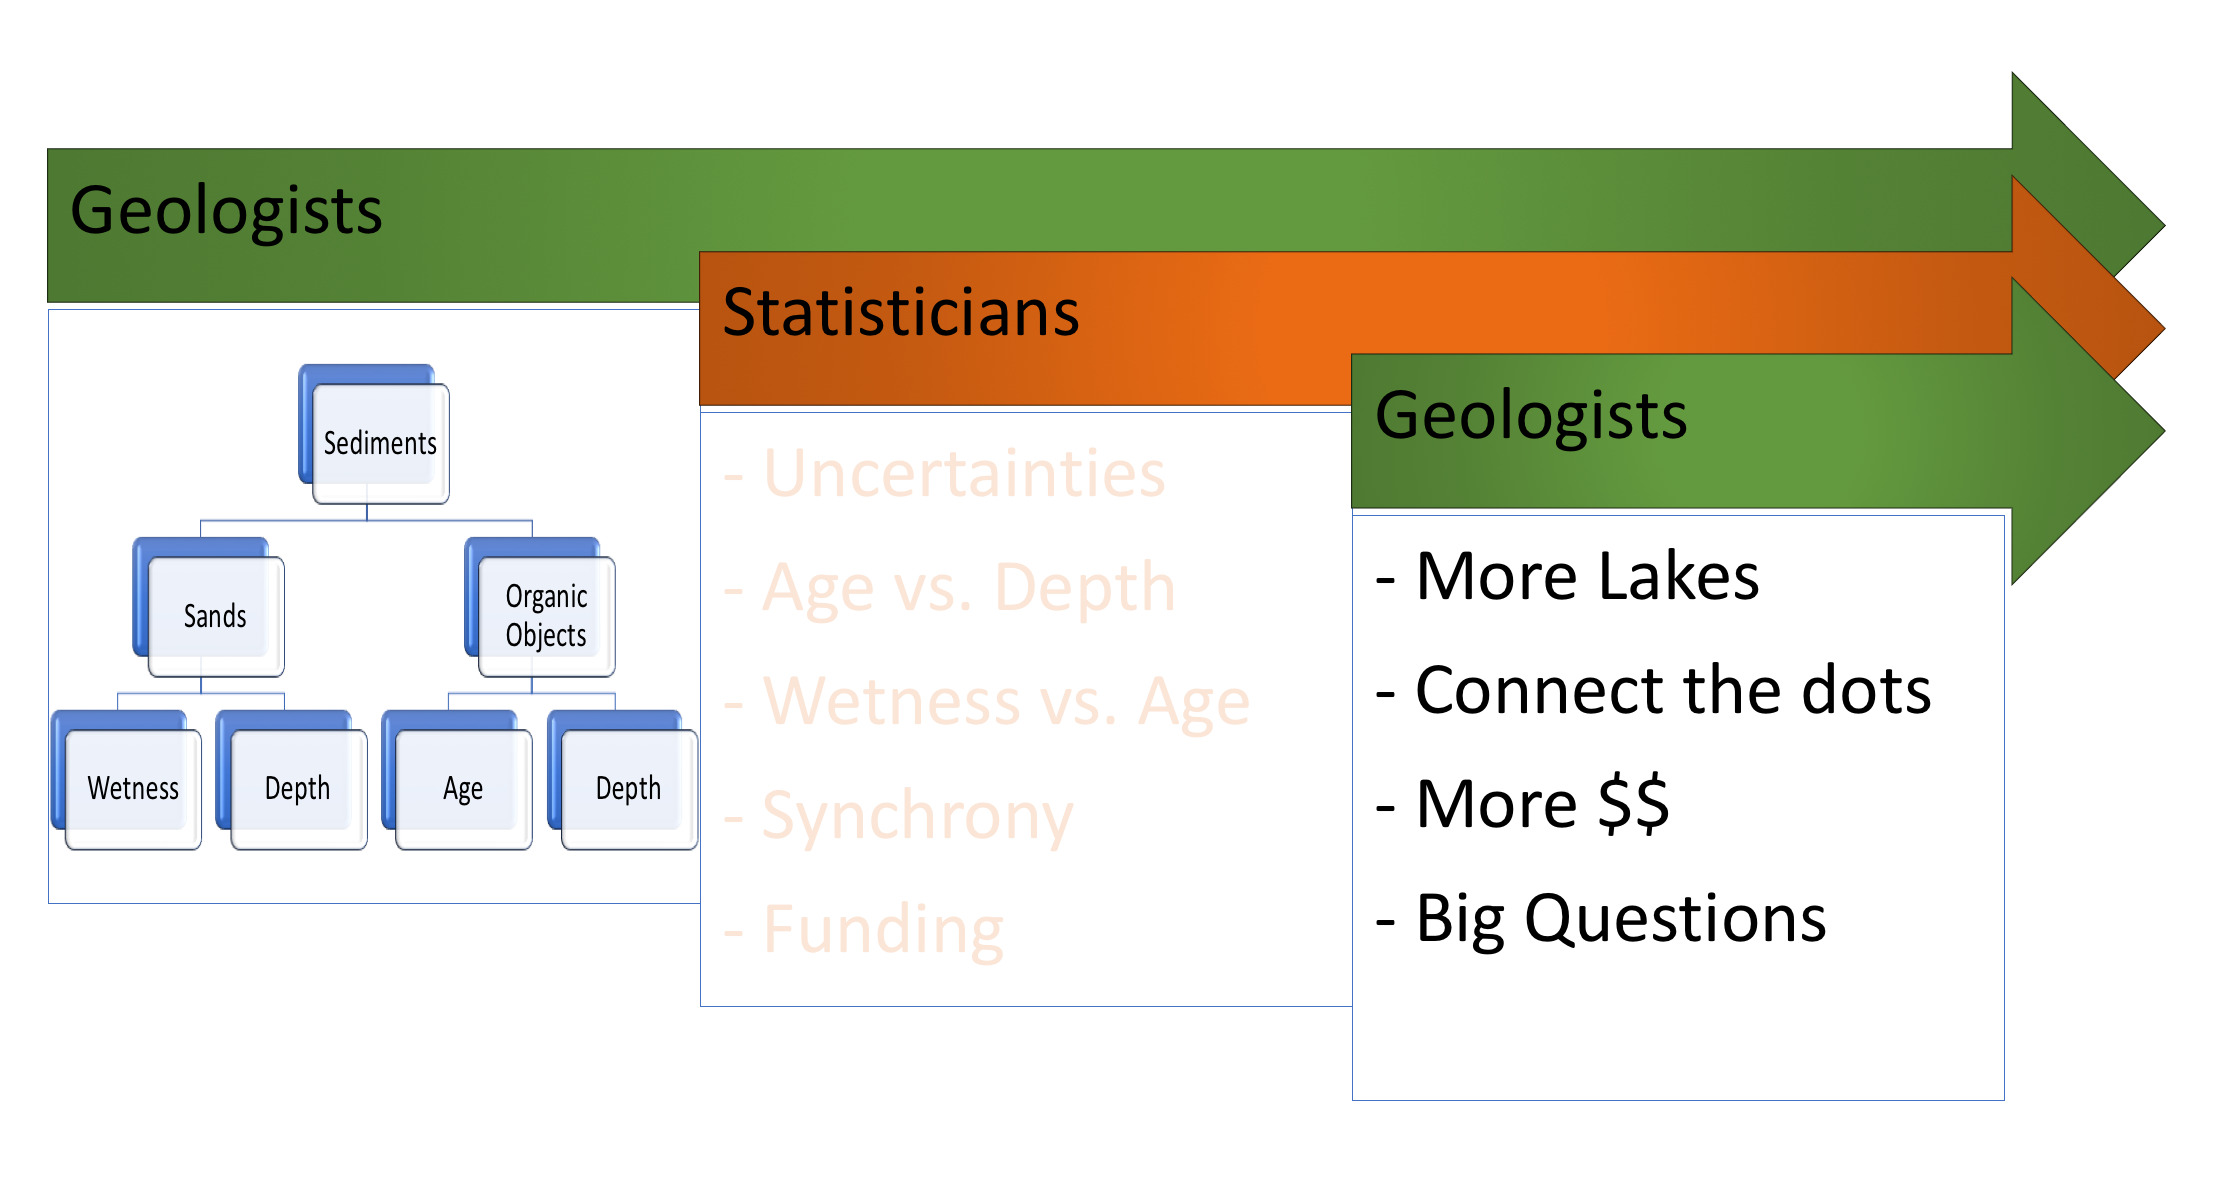
\includegraphics[width=1\textwidth]{page9}
\end{center}
}

\only<2>{
\vspace{-.3in}
\begin{center}
\hspace*{-.3in}
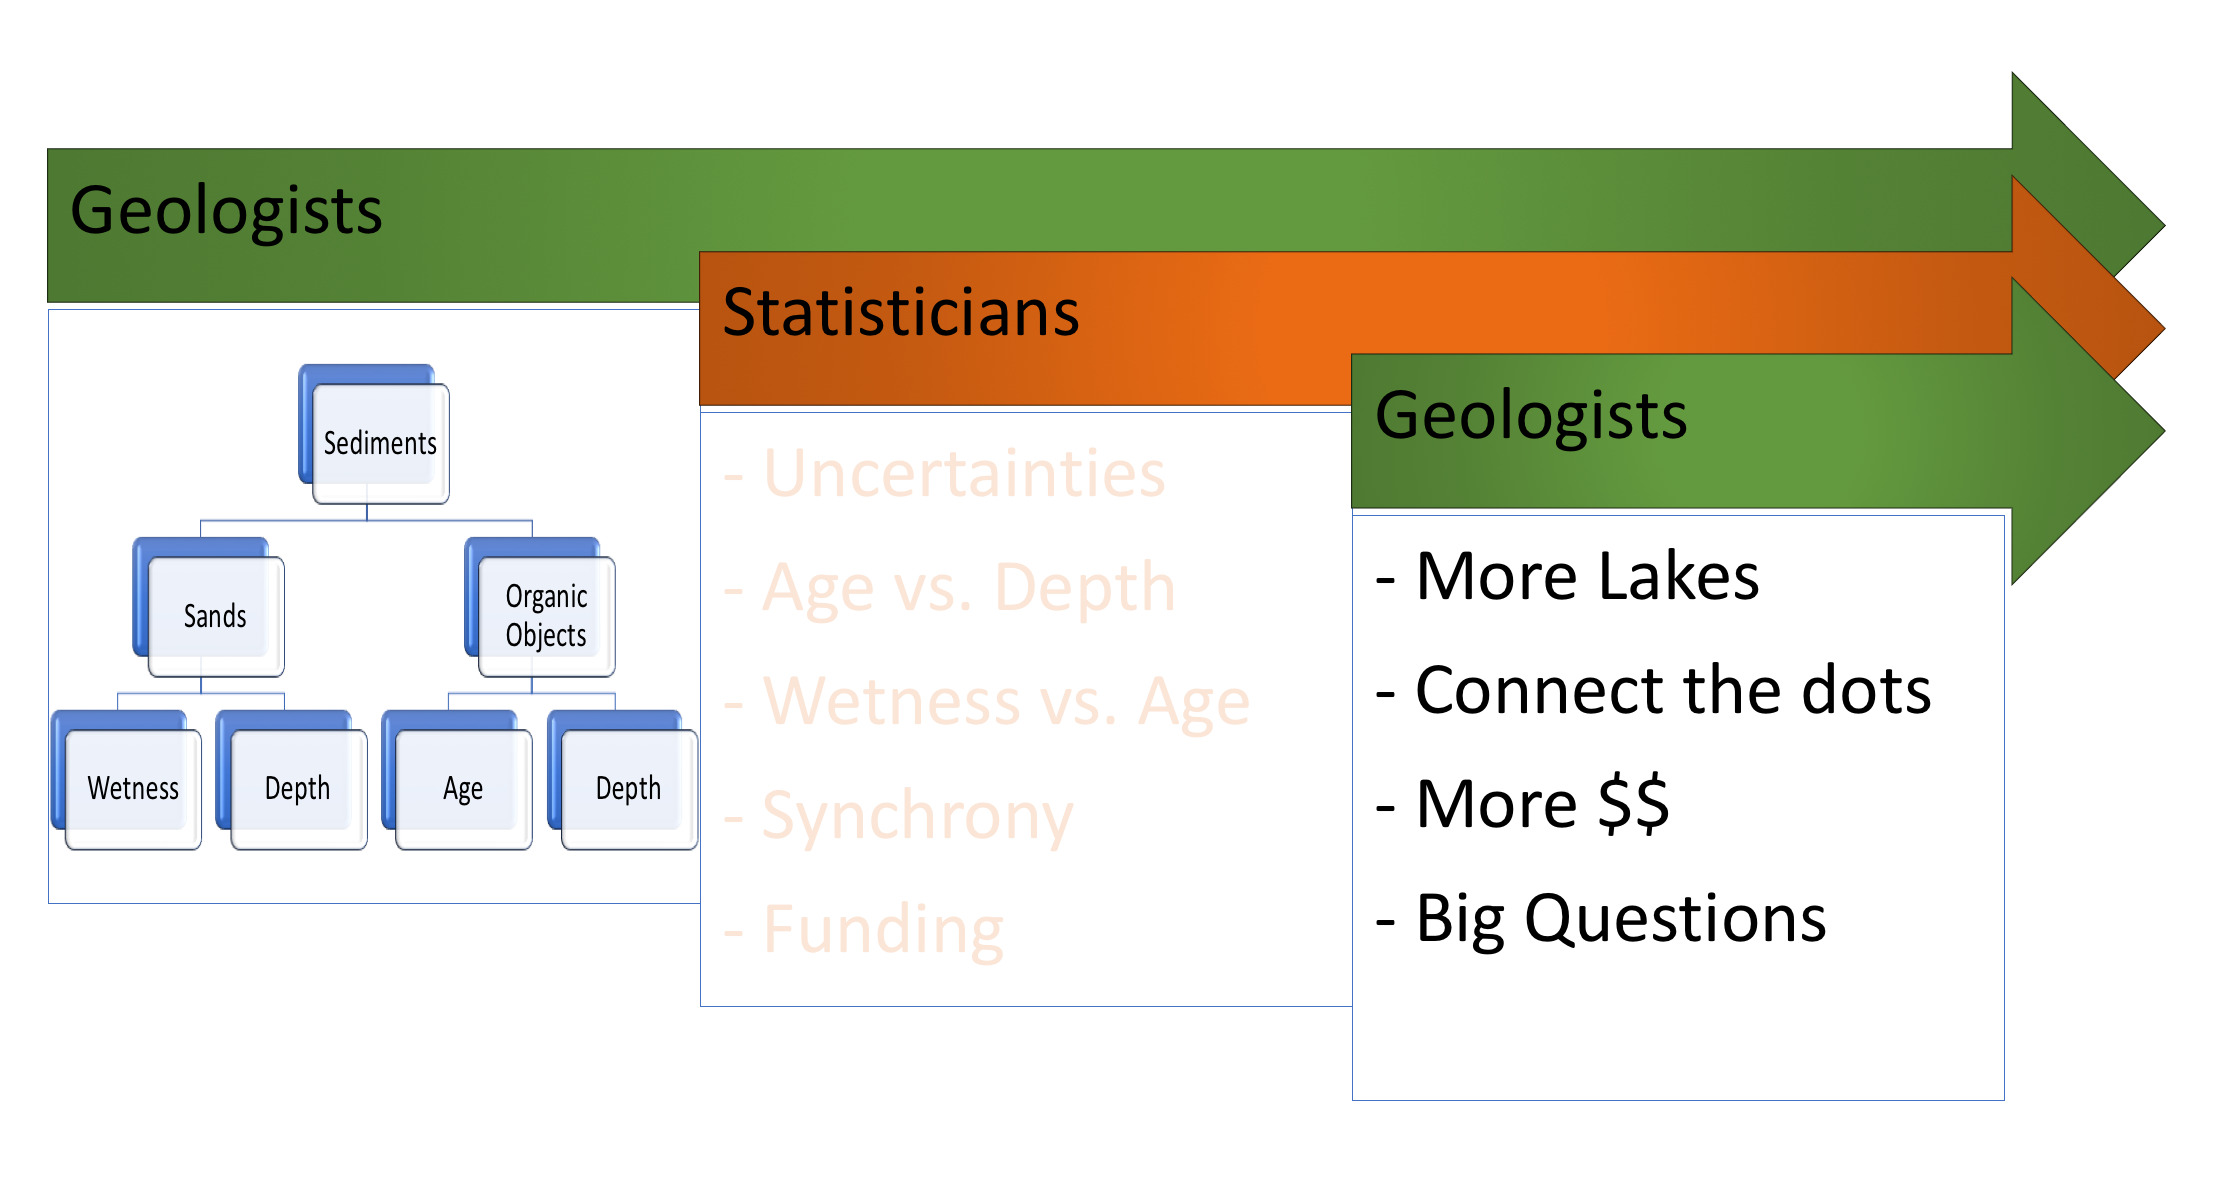
\includegraphics[width=1\textwidth]{page9}
\end{center}
}

\only<3>
{\begin{itemize}
	\item Depth $$ \bf D:=(d_1, d_2, \ldots, d_n)$$
	\item Temporal Location $$L := (\ell_1,\ell_2,\ldots, \ell_k)$$
	\item Wetness $$ W \bf (D):=\big(w(d_1), w(d_2) ,\ldots, w(d_n)\big)$$
  \end{itemize}
  $\widehat{V_i}(\ell_k)$ represents the $i^{th}$ estimate of wetness at time $\ell_k$
  $$\widehat{V_i}(\ell_k) = \frac{\sum_{j=1}^{n} K_h(|| t_i|d_j - \ell_k ||) w(d_j)}{\sum_{j=1}^{n} K_h(|| t_i|d_j - \ell_k ||) }$$
  }



\only<4>
{\begin{figure}
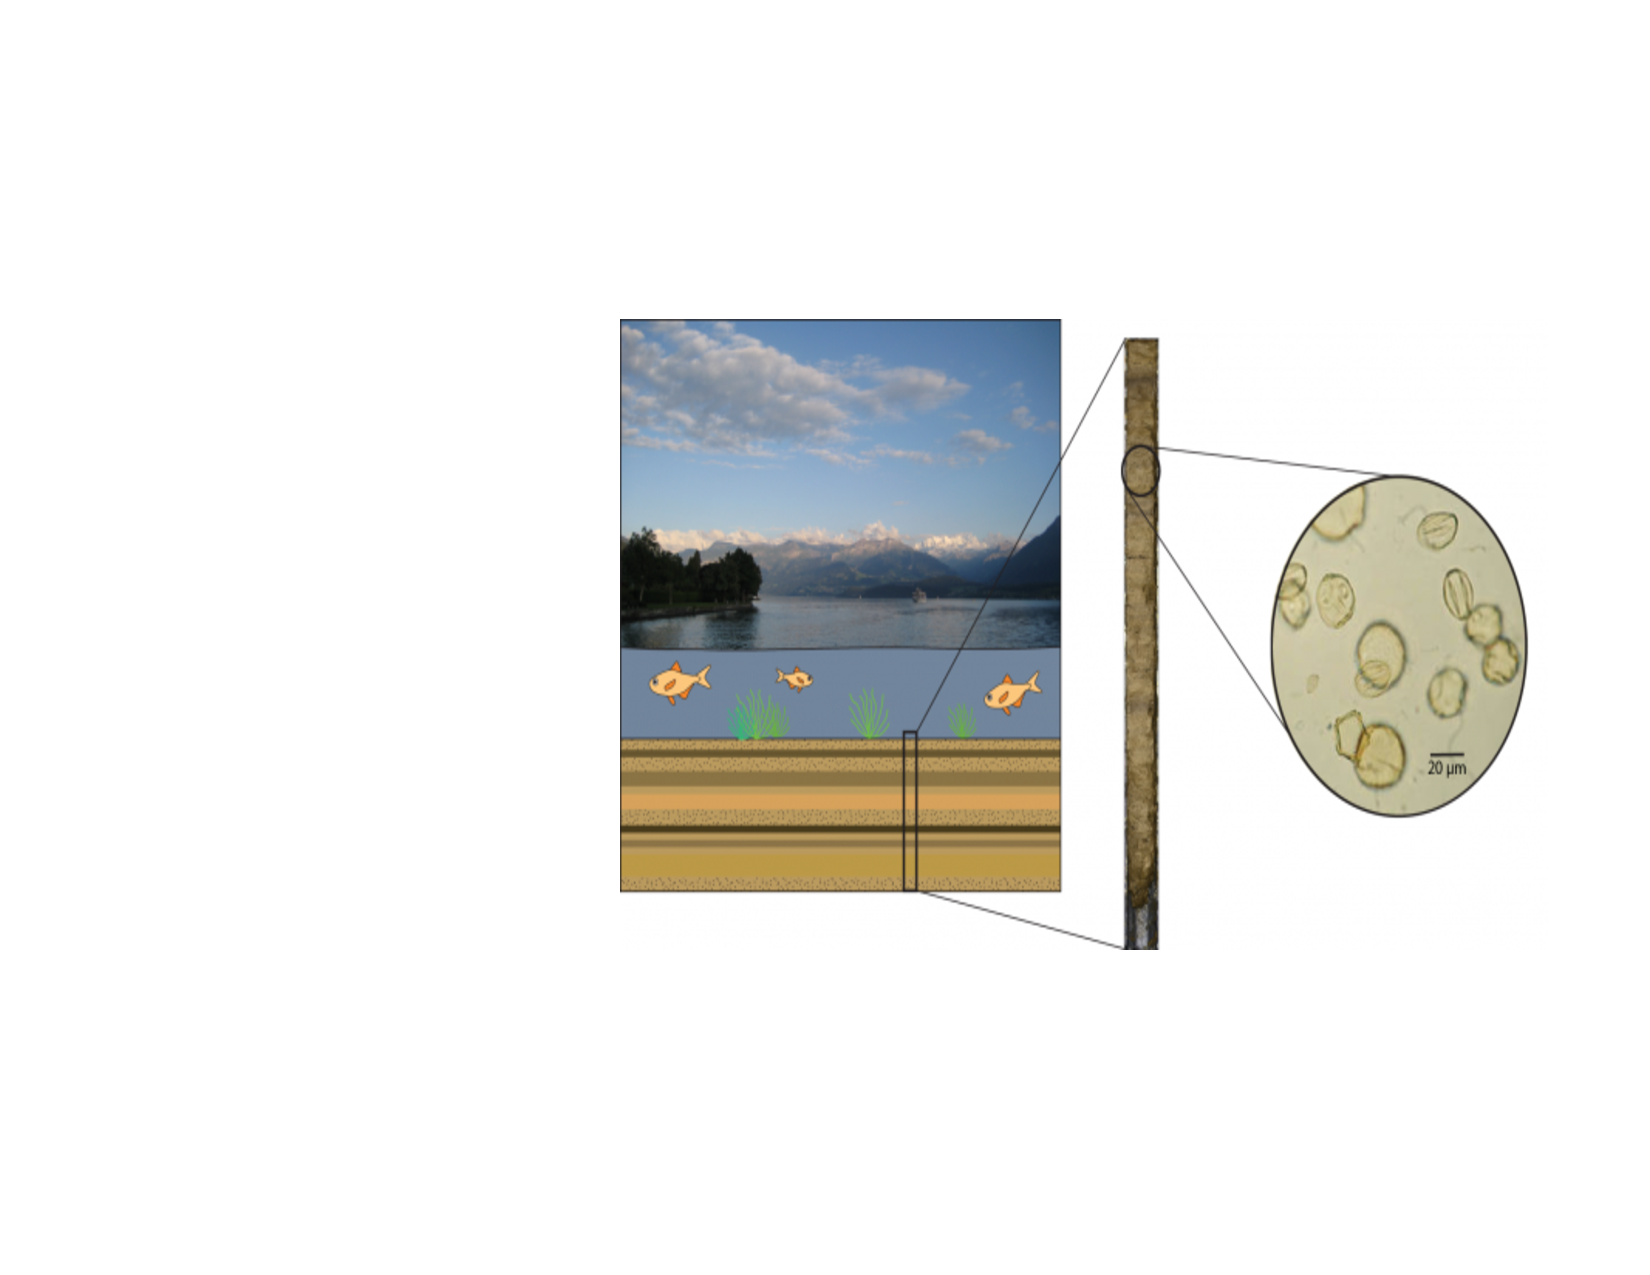
\includegraphics[width=.5\linewidth]{cores.pdf}
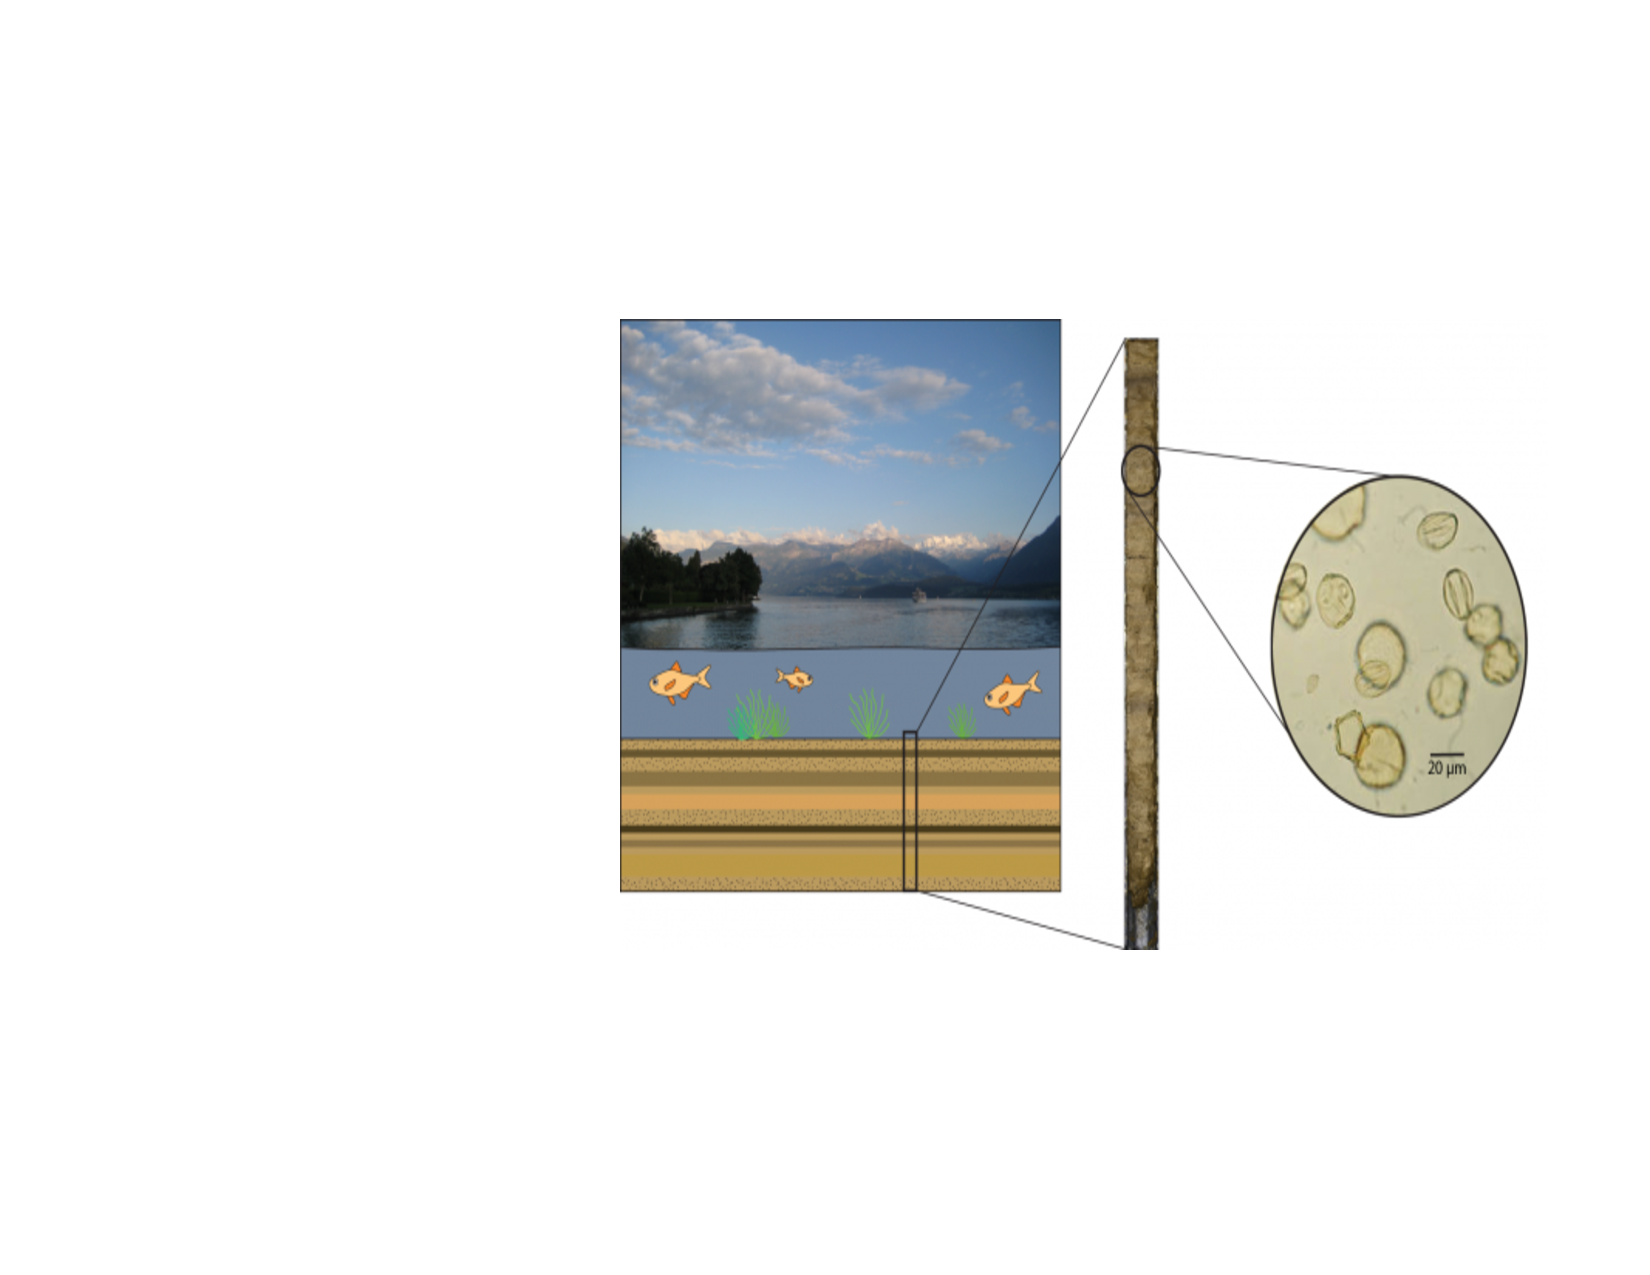
\includegraphics[width=.5\linewidth]{cores.pdf}
\end{figure}}




\end{frame}




\section{Findings}
\subsection{Climate Synchrony}






\begin{frame}


\only<1>{
\vspace{-.3in}
\begin{center}
\hspace*{-.3in}
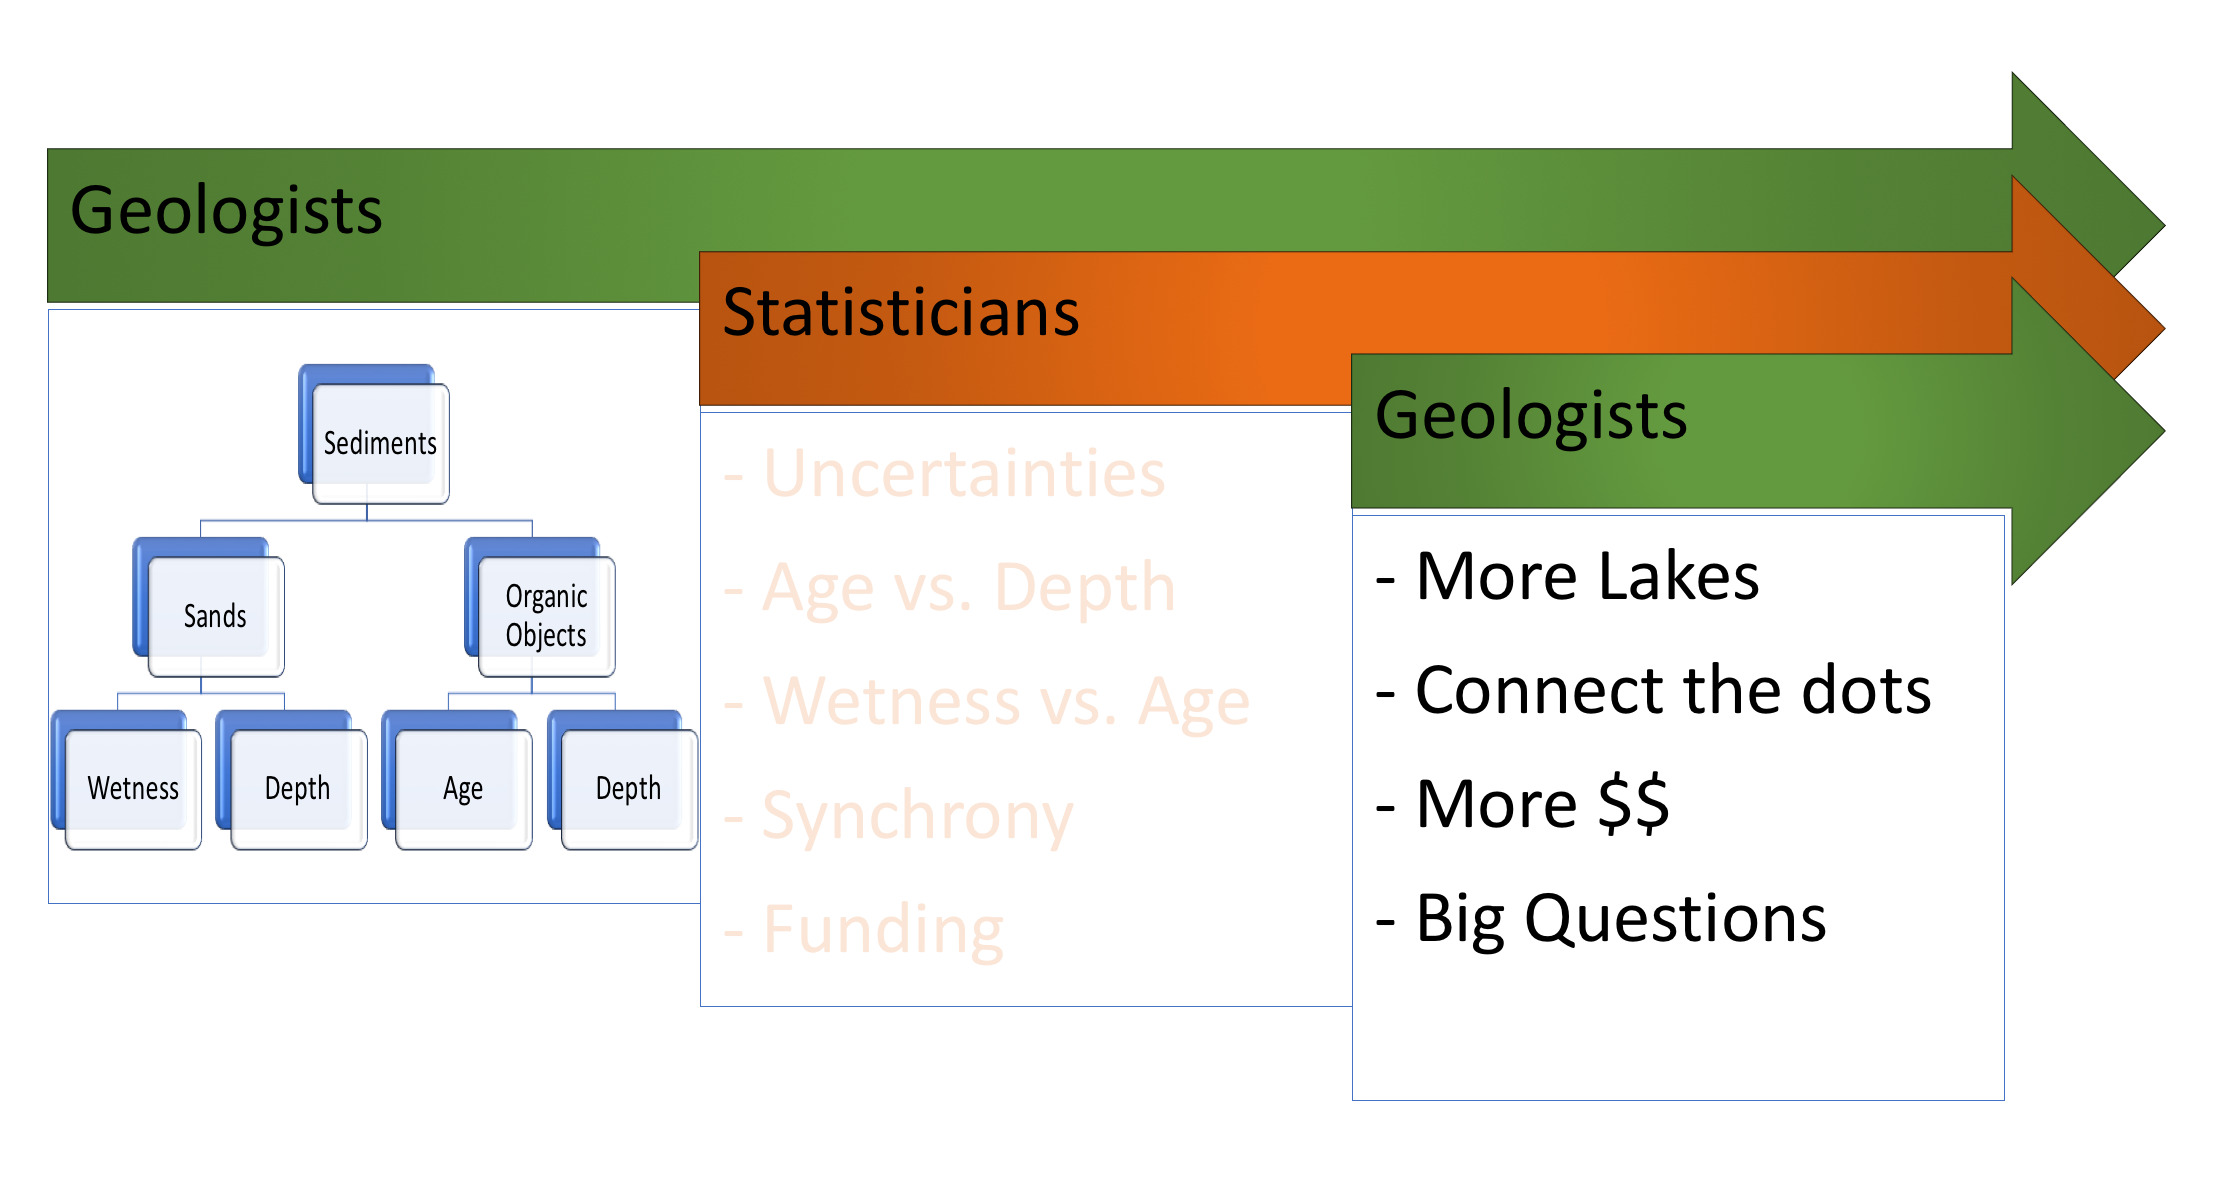
\includegraphics[width=1\textwidth]{page9}
\end{center}
}

\only<2>{
\vspace{-.3in}
\begin{center}
\hspace*{-.3in}
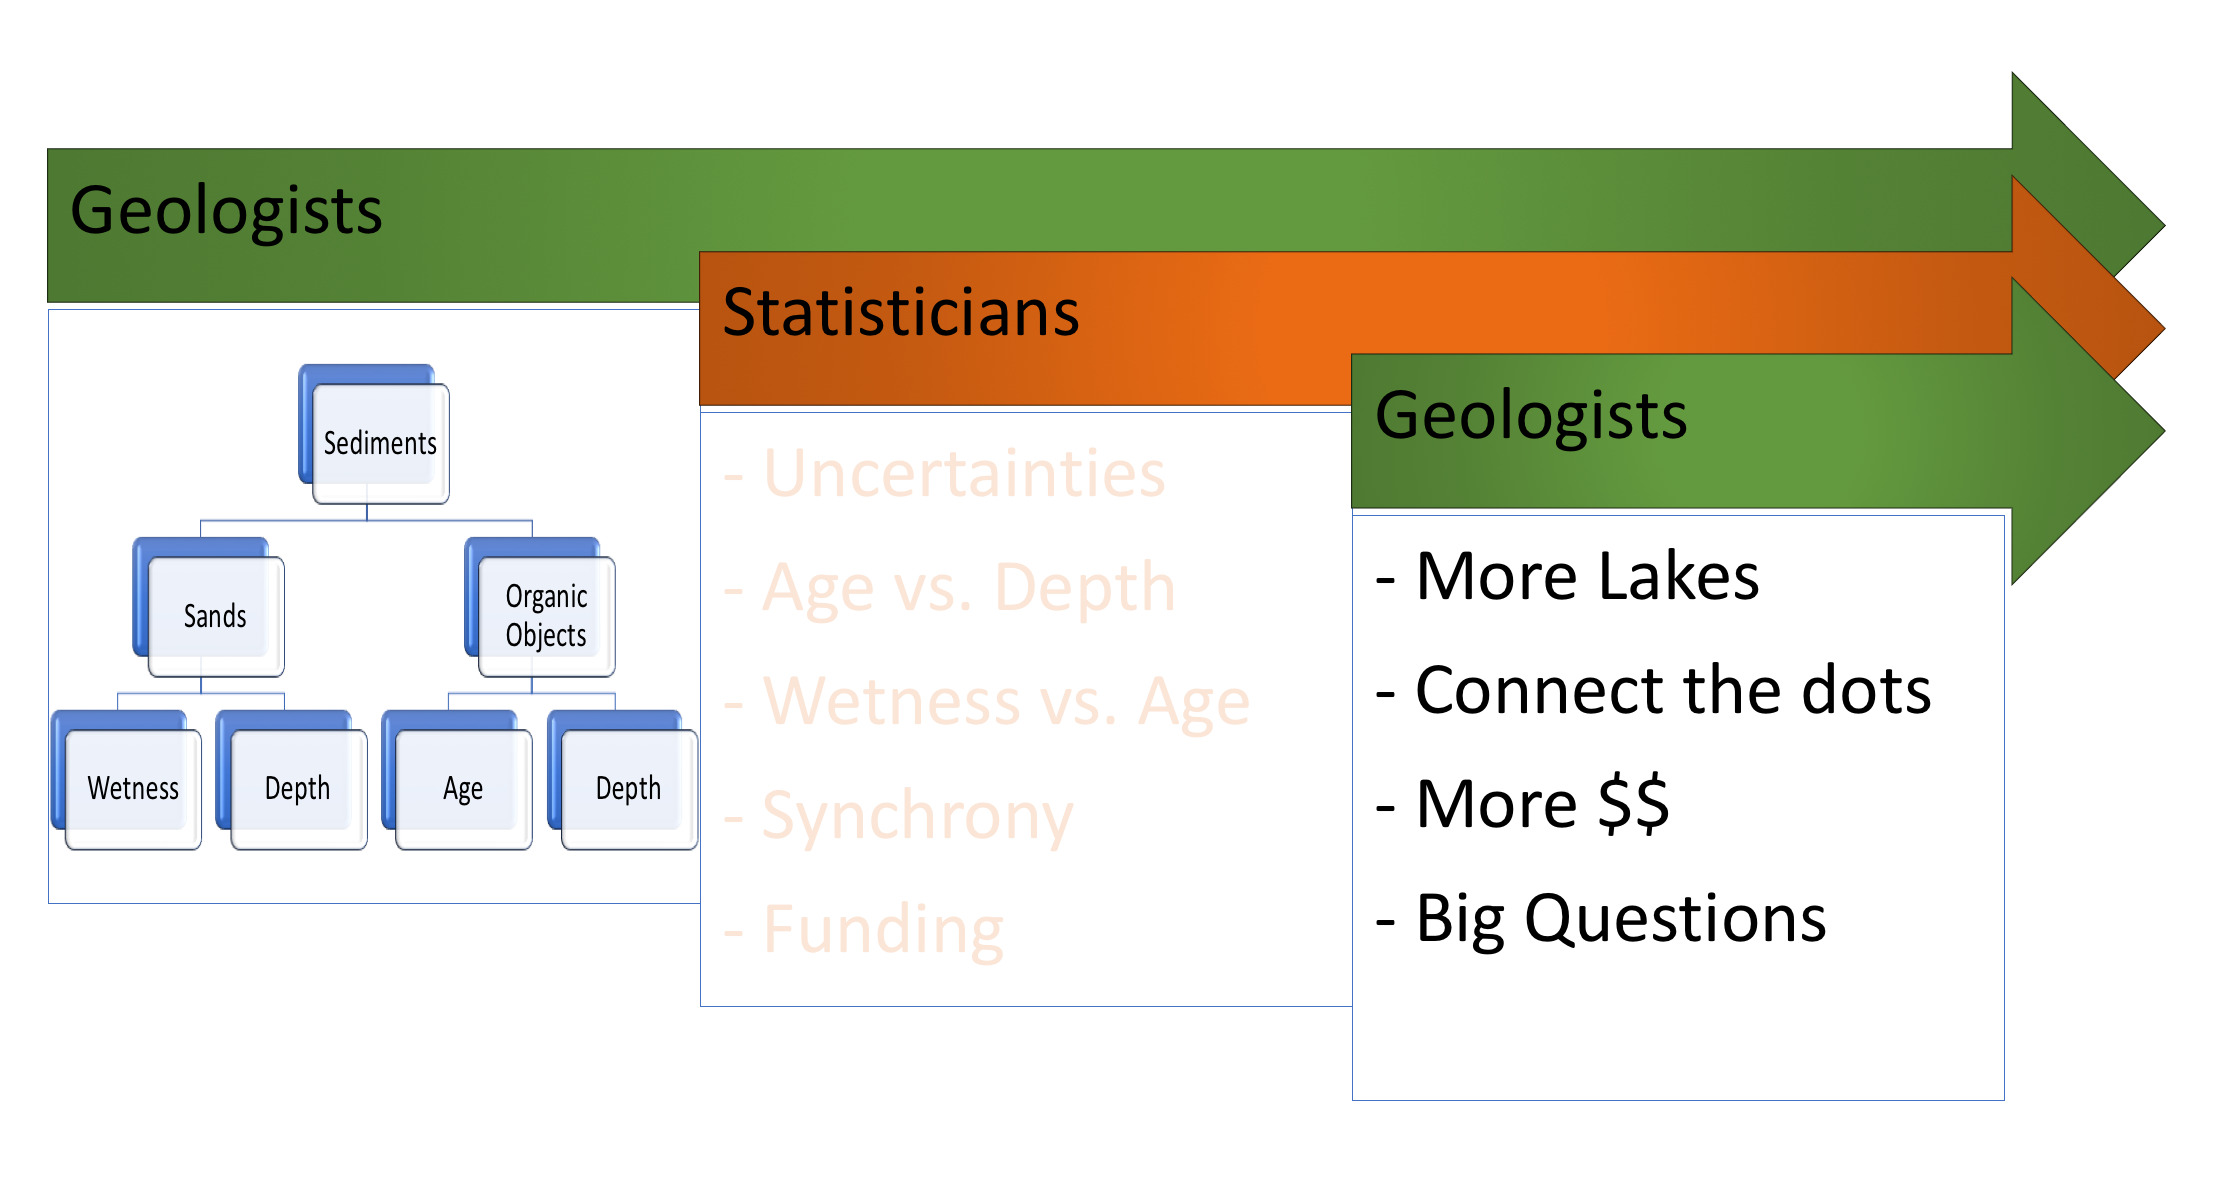
\includegraphics[width=1\textwidth]{page9}
\end{center}
}

\only<3>{
\begin{figure}
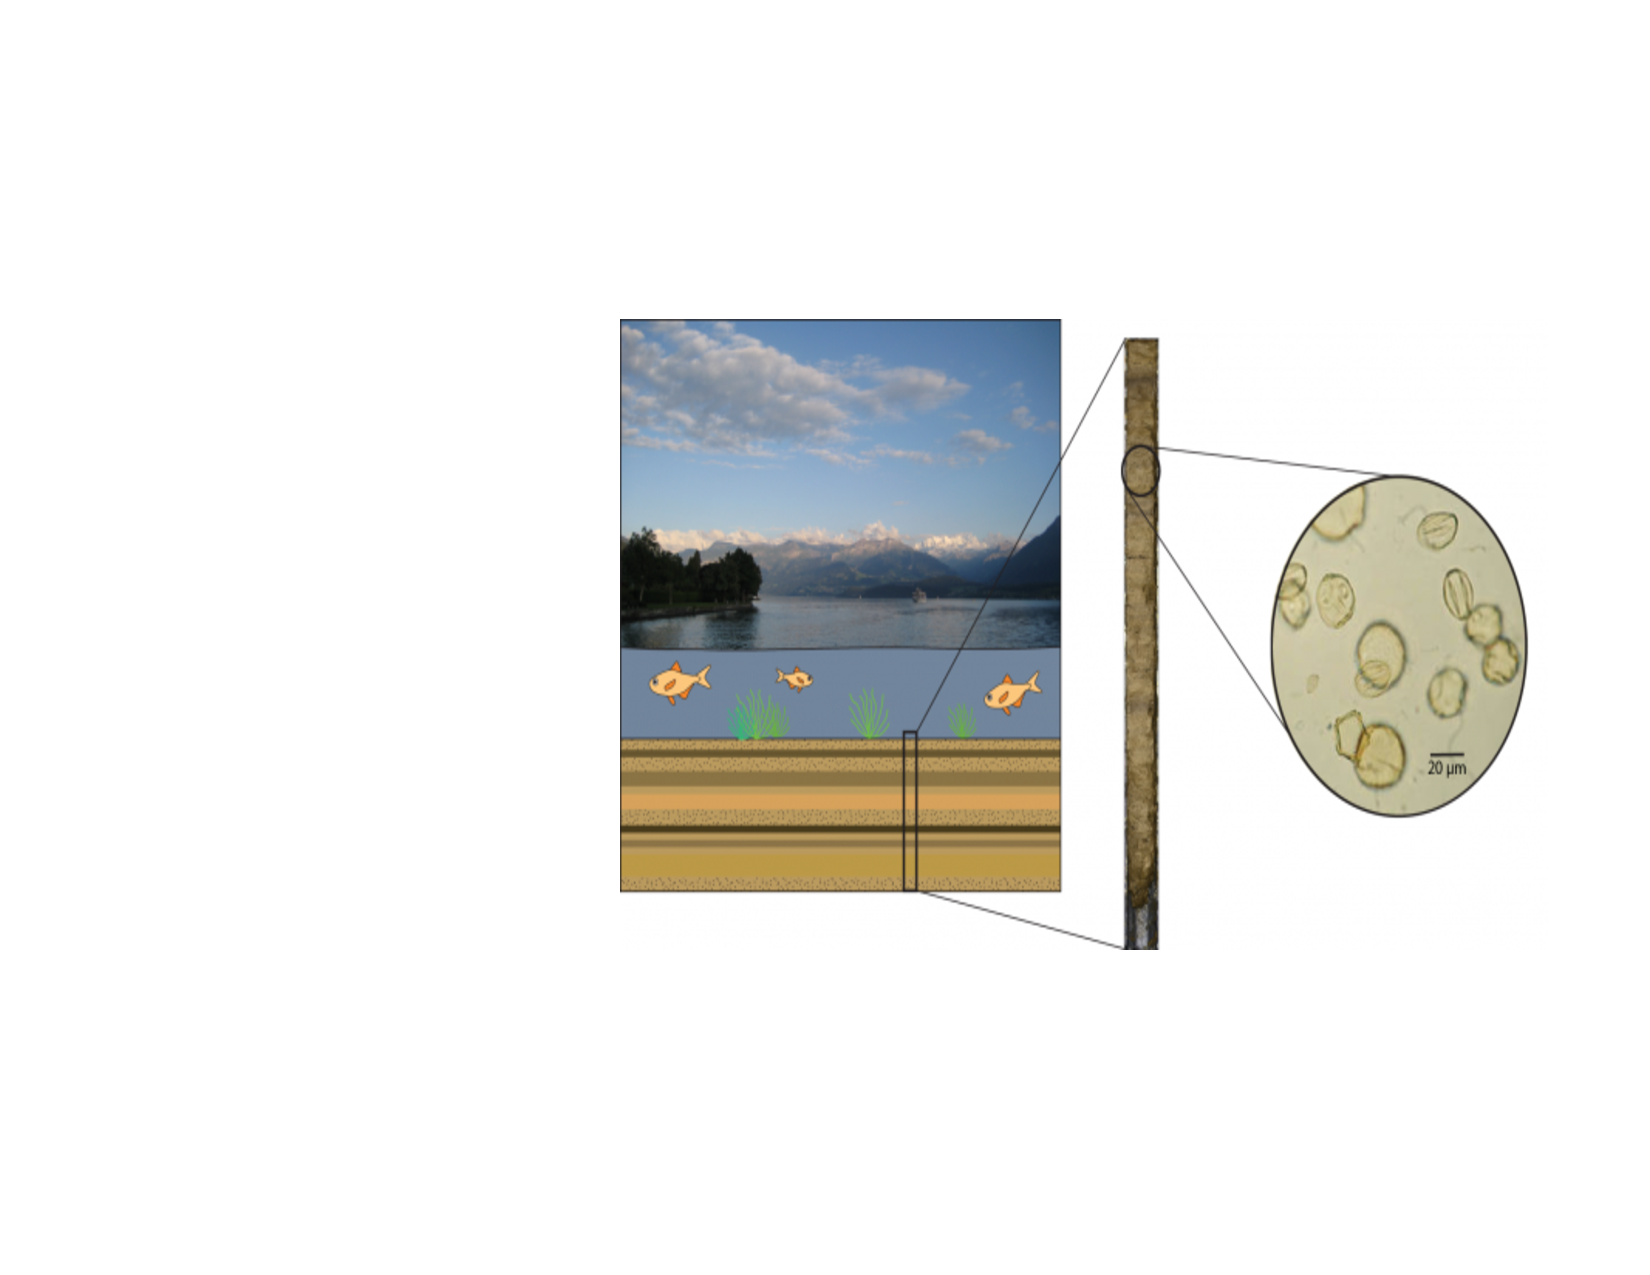
\includegraphics[width=.5\linewidth]{cores.pdf}
\pause
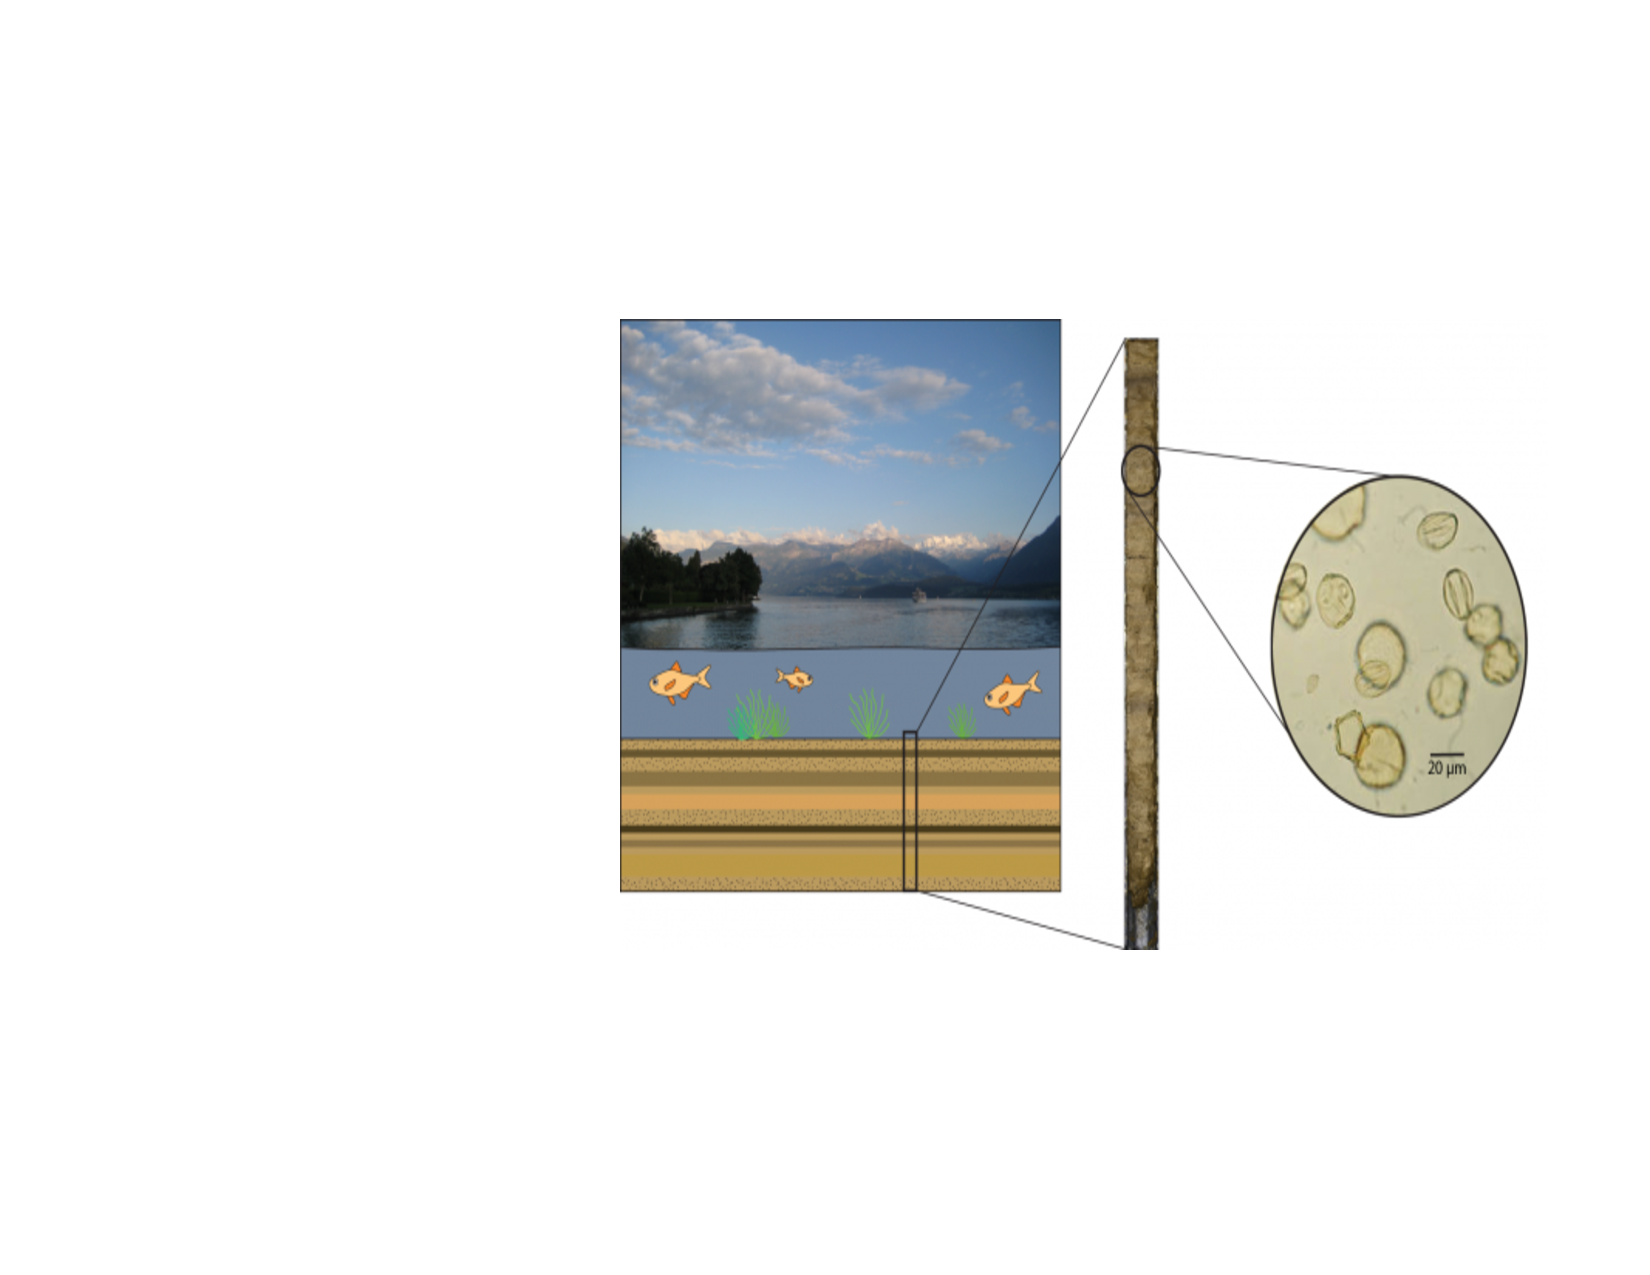
\includegraphics[width=.5\linewidth]{cores.pdf}
\end{figure}}
\frametitle{Synchrony}
\end{frame}






\subsection{Dipole}
\begin{frame}
\frametitle{Climatic Dipole}
\begin{itemize}
\item<1-> \textbf{Definition: }Latitude dividing two diverging weather systems
\begin{figure}
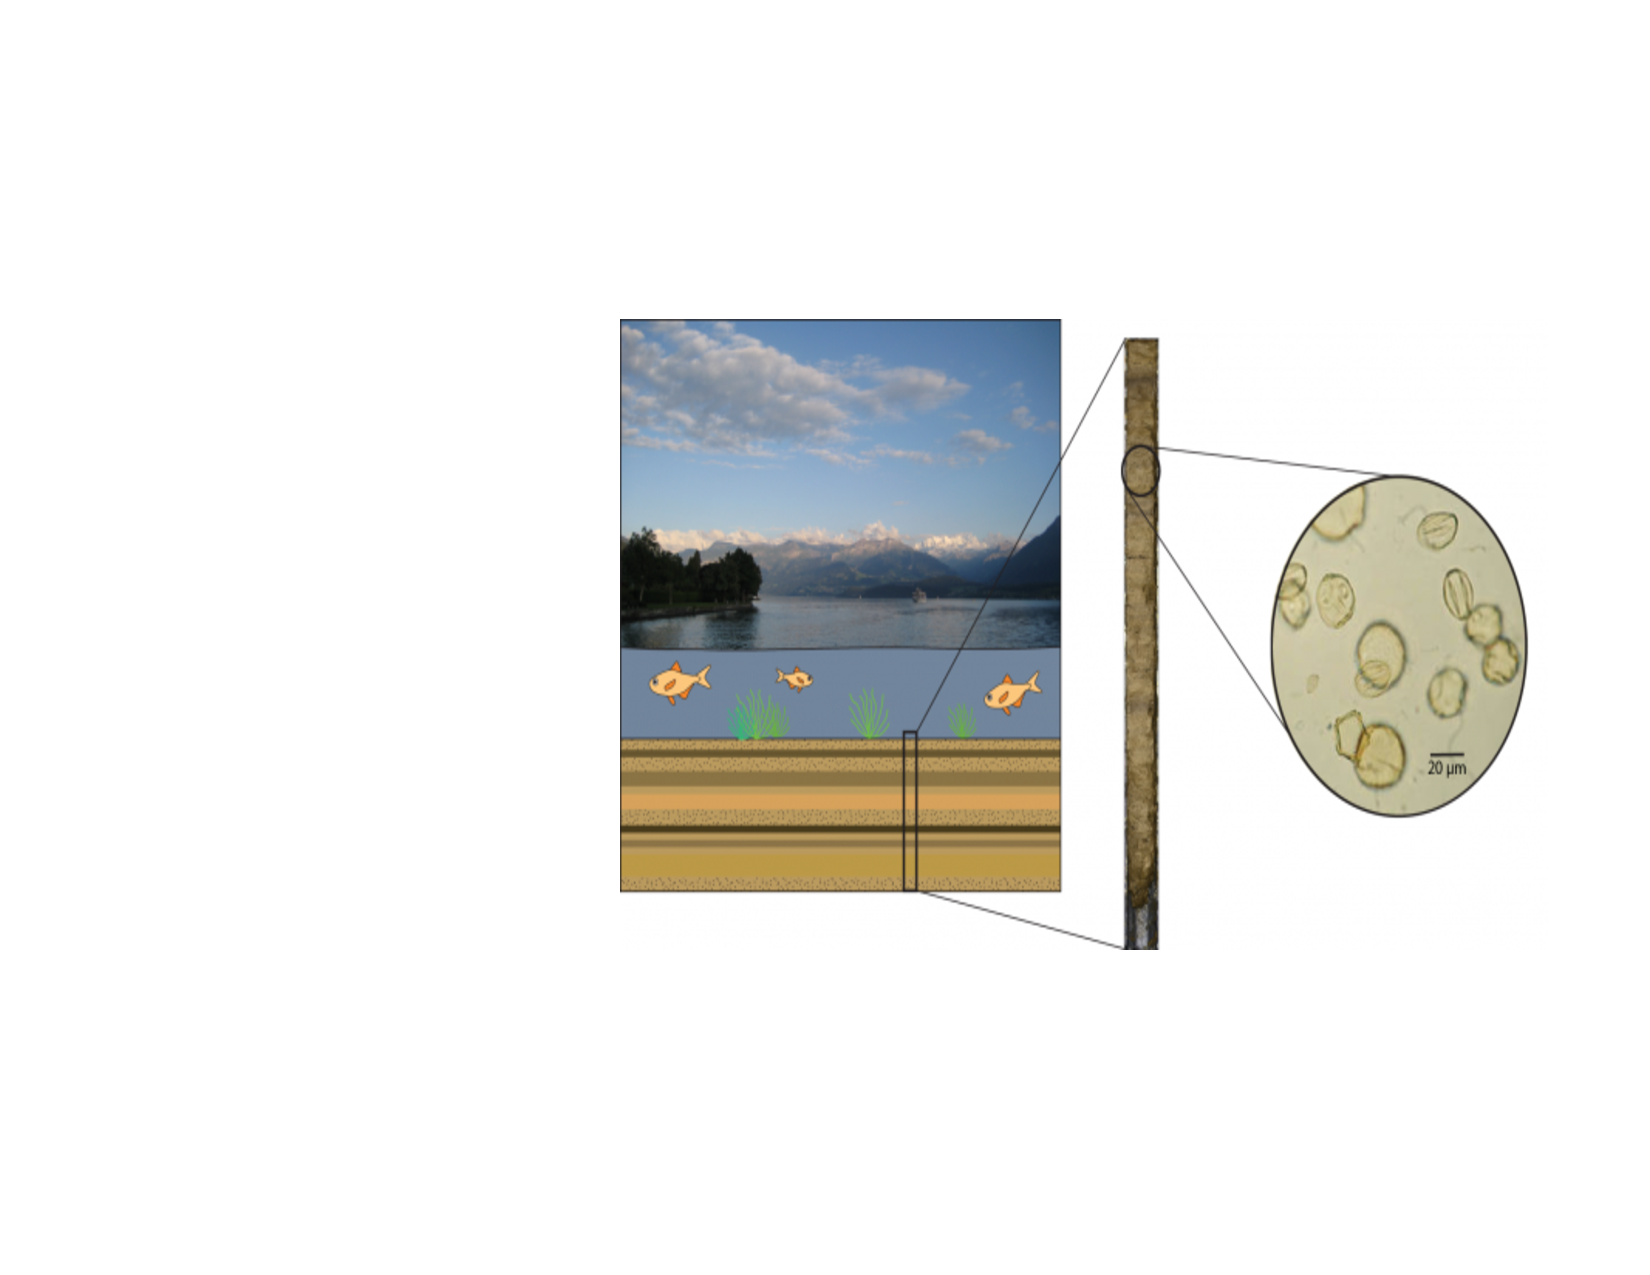
\includegraphics[width=.49\linewidth]{cores.pdf}
\end{figure}
\item<2-> \textbf{Characteristics: }
	\begin{itemize}
	\item Shifts
    \item Might be a reason for climate change
	\end{itemize}
\end{itemize}
\end{frame}







\subsection{Sample Size Effects}
\begin{frame}
\frametitle{Deteriorated Features}


\only<1>{
\vspace{-.3in}
\begin{center}
\hspace*{-.3in}
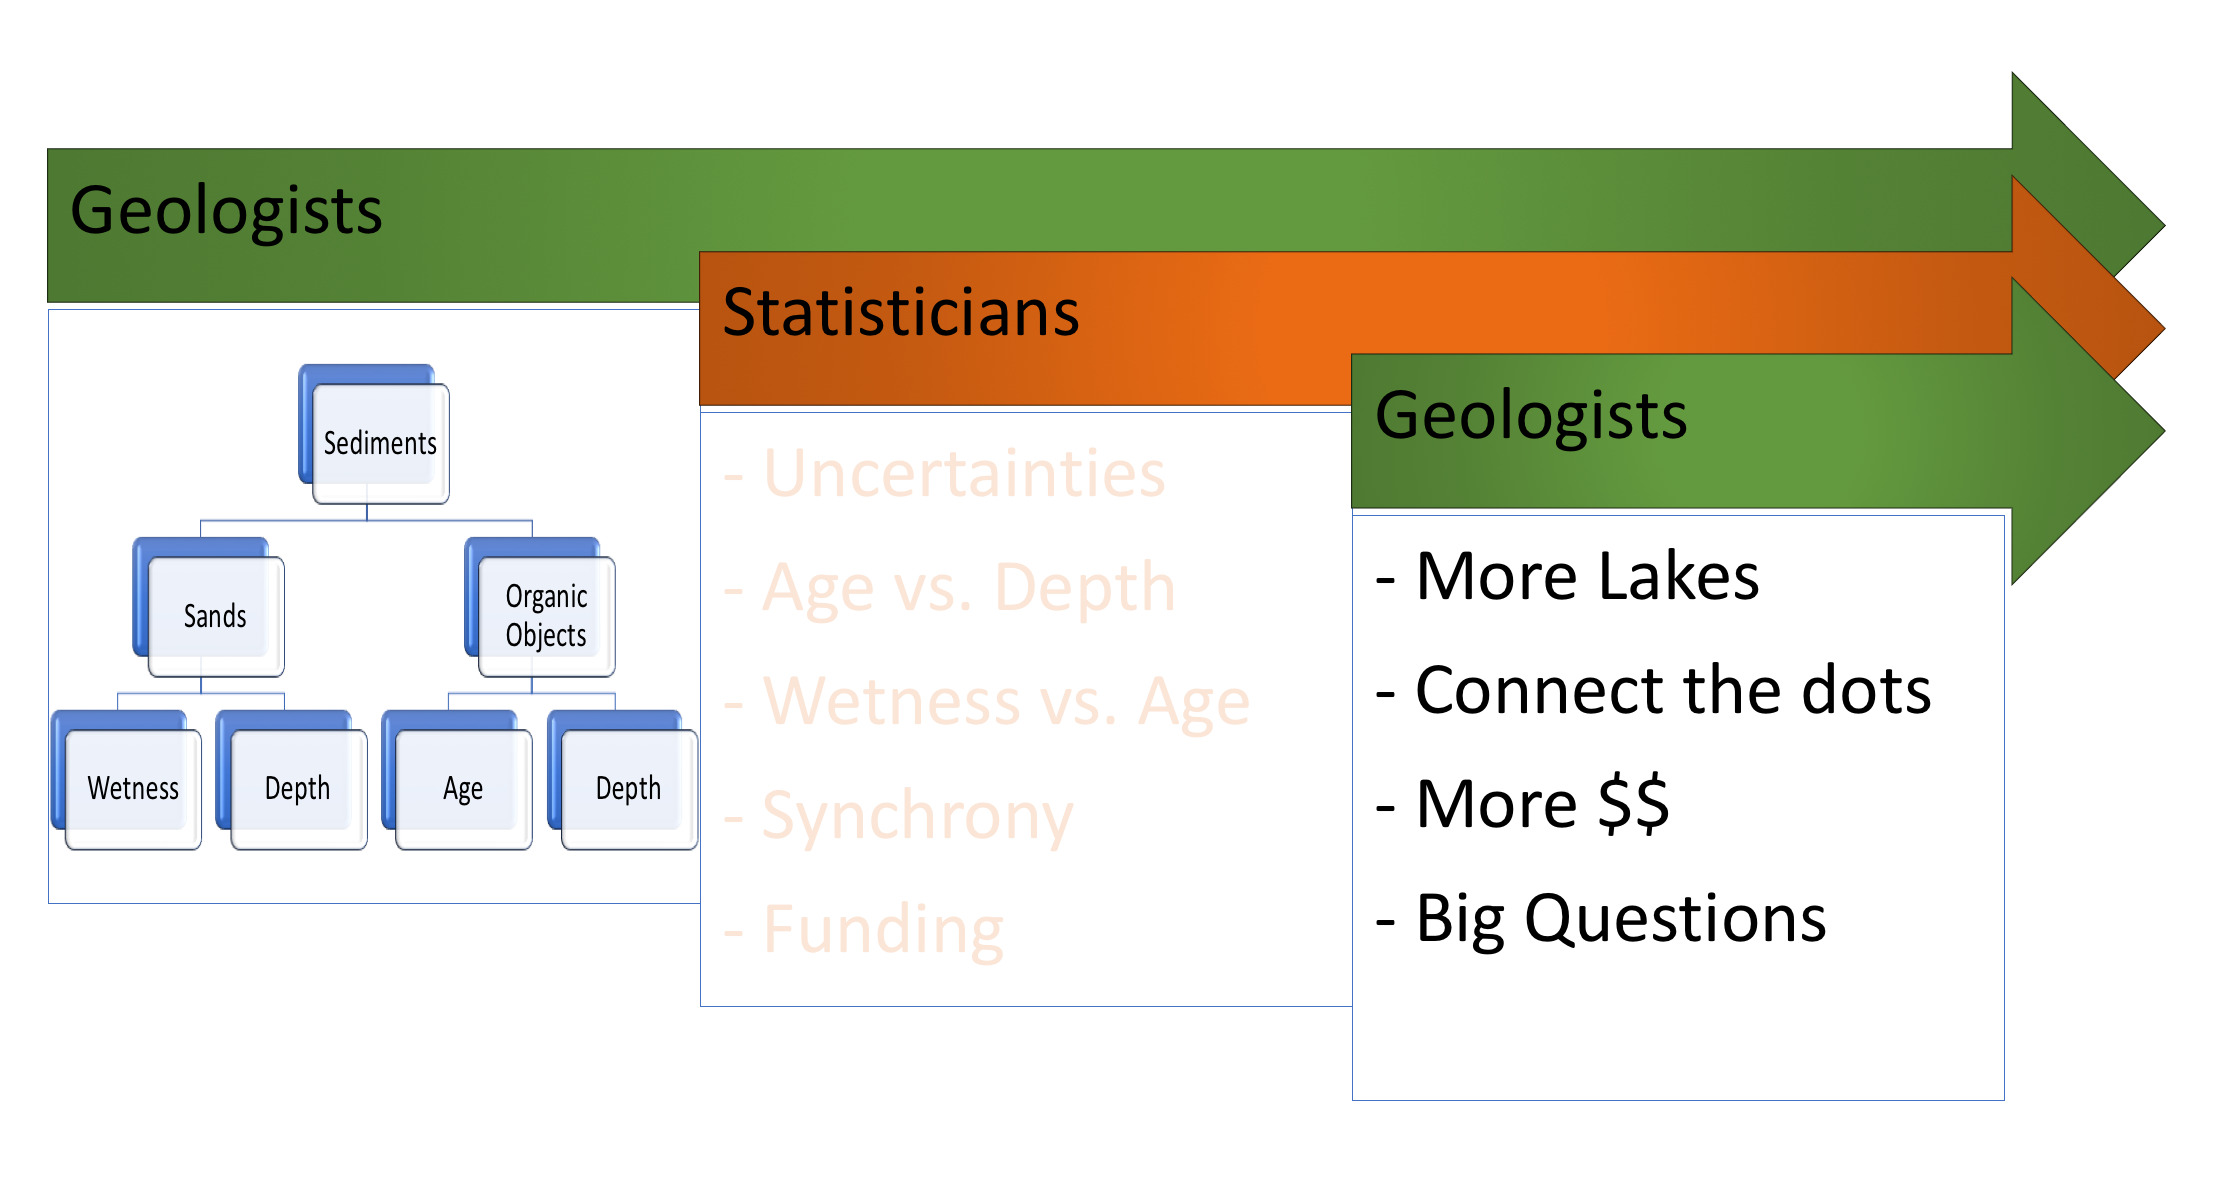
\includegraphics[width=1\textwidth]{page9}
\end{center}
}

\only<2>{
\vspace{-.3in}
\begin{center}
\hspace*{-.3in}
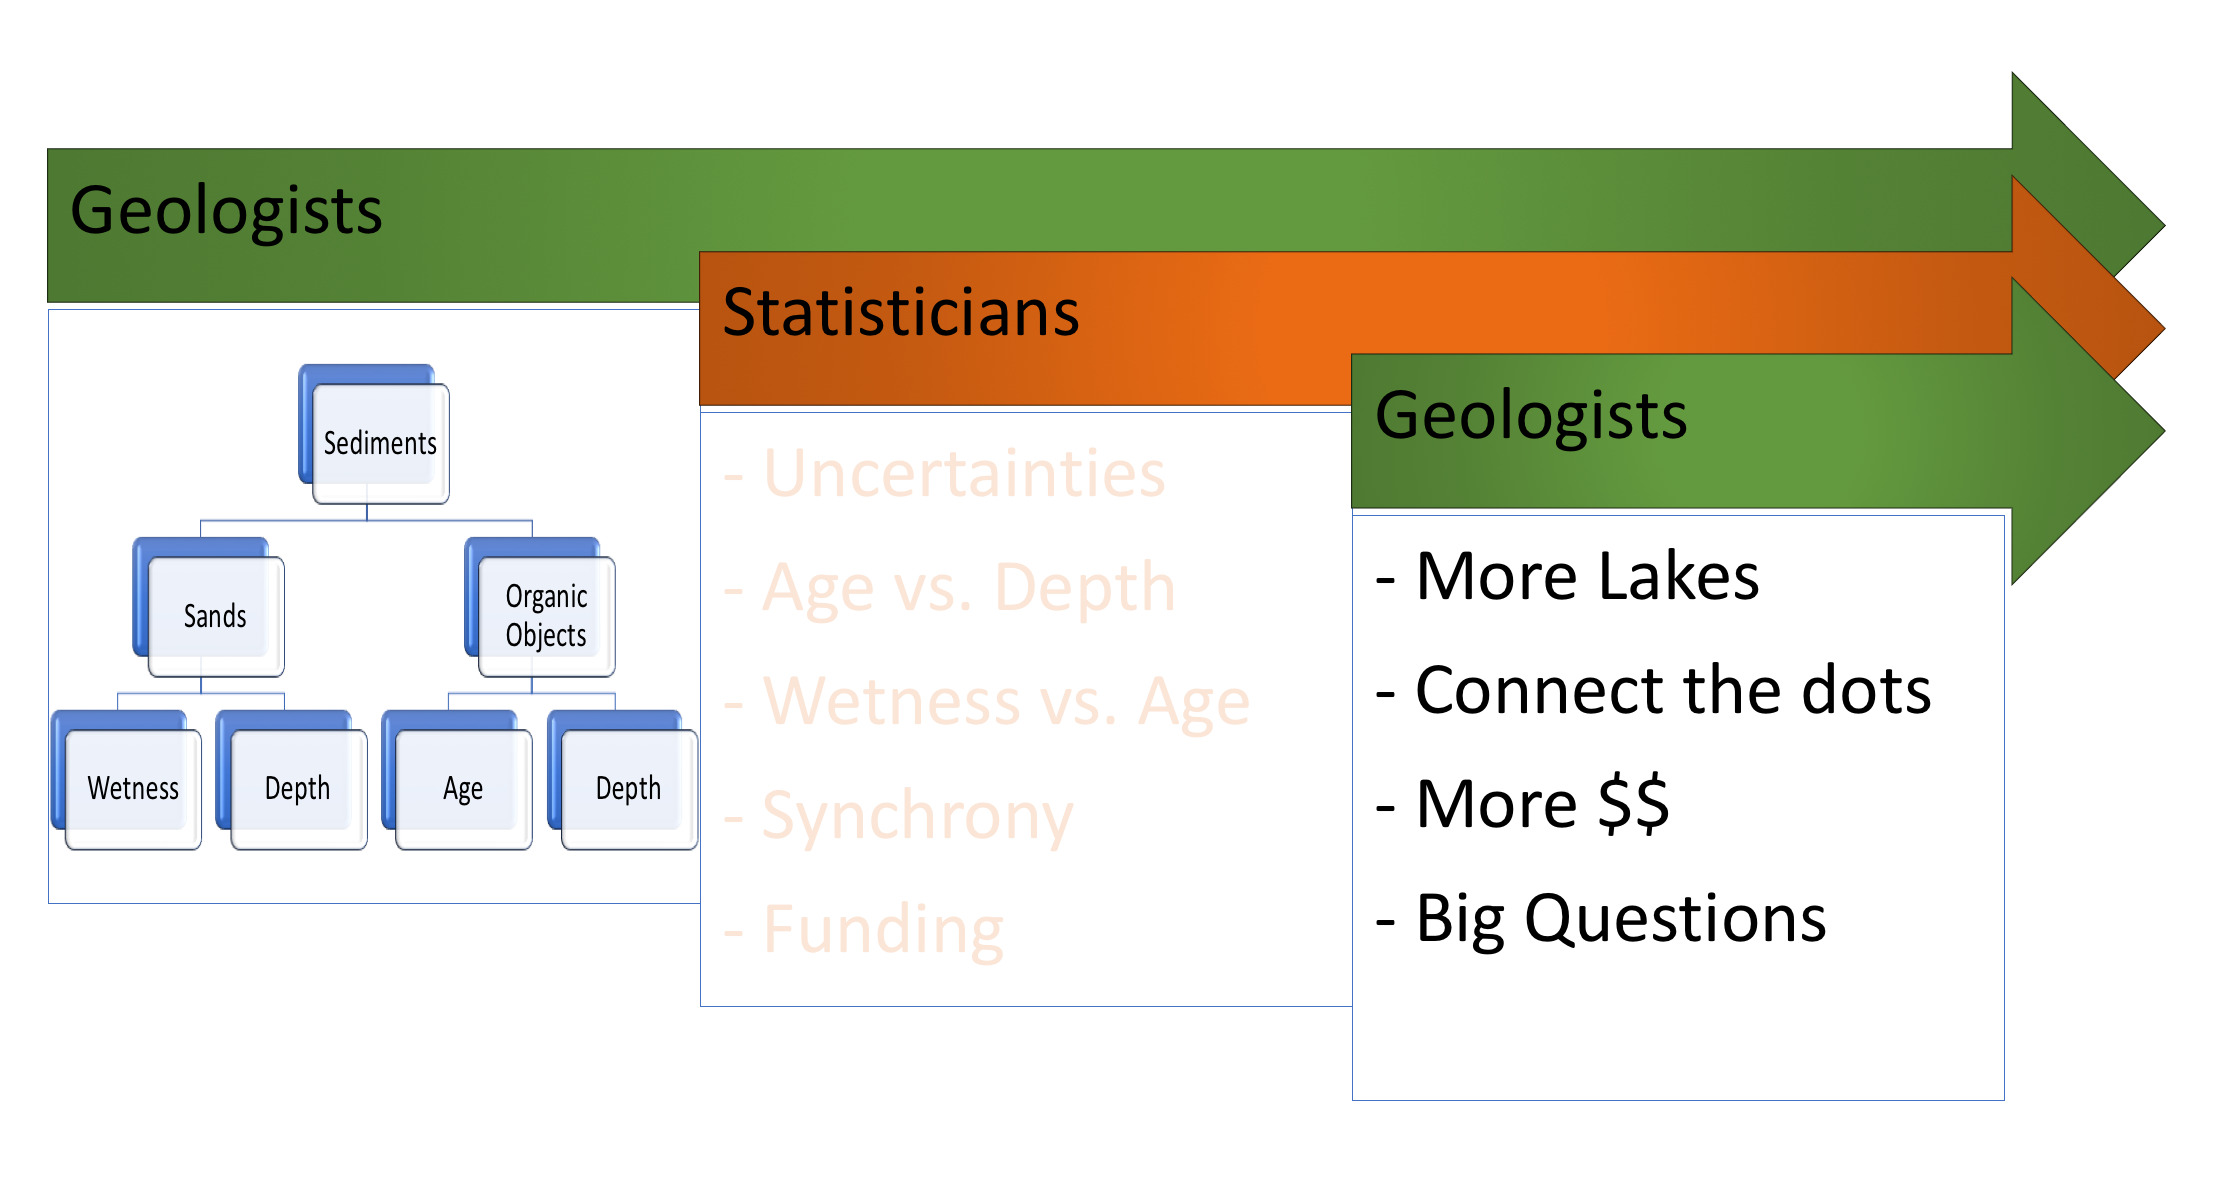
\includegraphics[width=1\textwidth]{page9}
\end{center}
}


\only<3>{
\begin{figure}
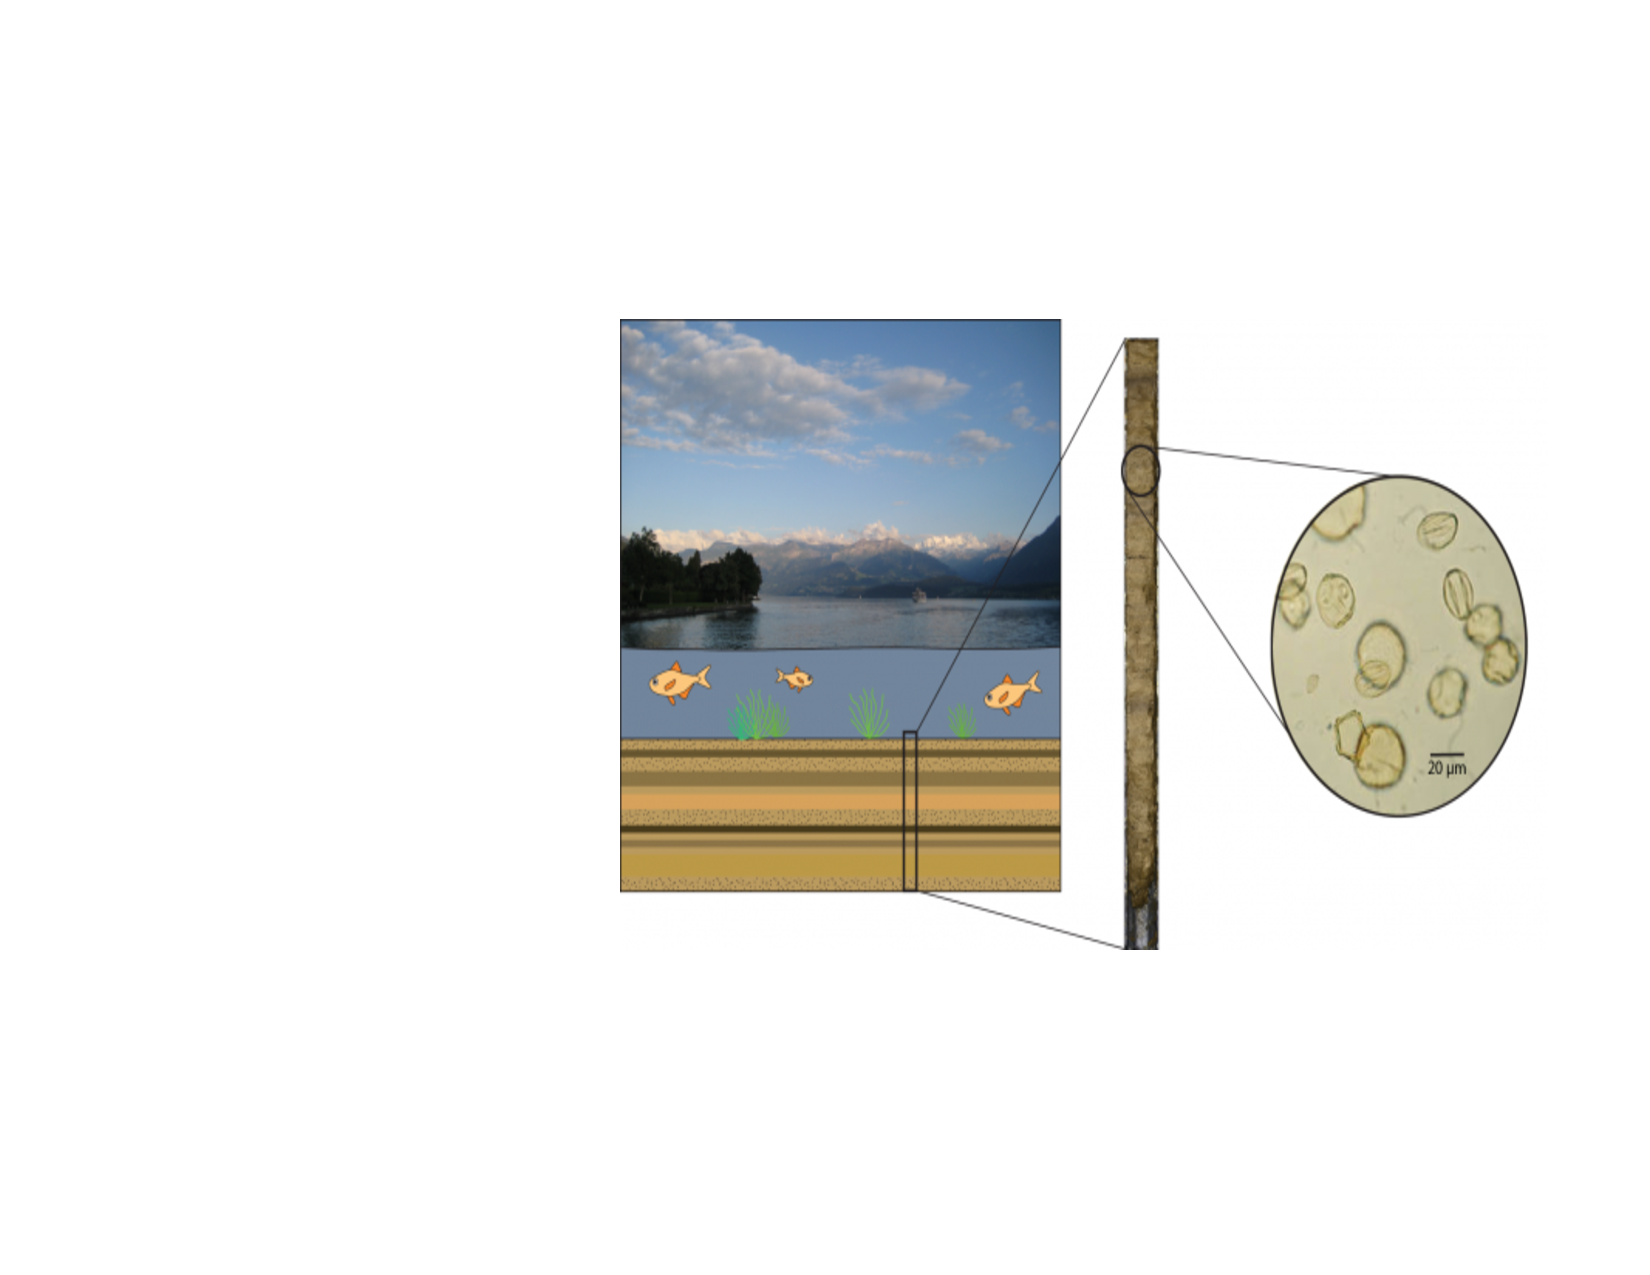
\includegraphics[width=.8\linewidth]{cores.pdf}
\end{figure}}
\end{frame}







\begin{frame}
\frametitle{Deterioration of the Variance}

\only<1>
{\begin{figure}
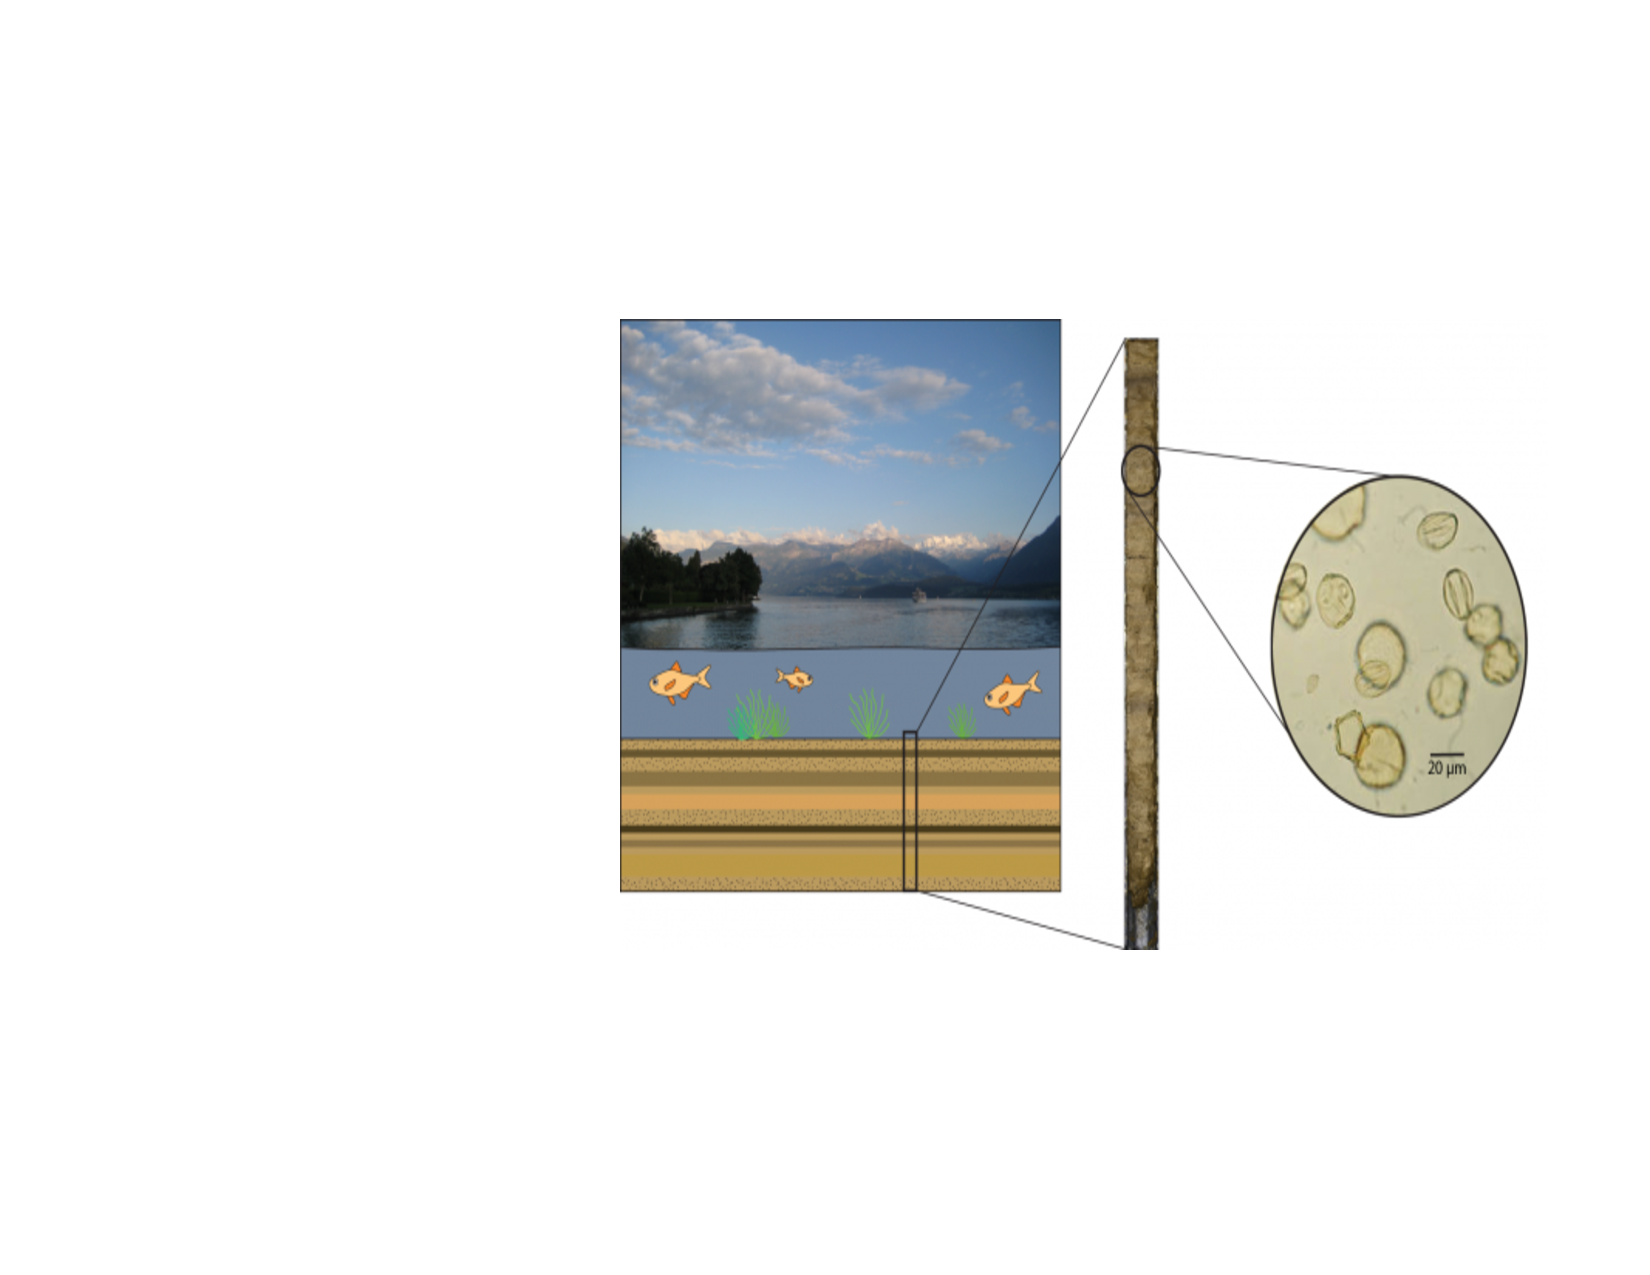
\includegraphics[width=.65\linewidth]{cores.pdf}
\end{figure}}

\only<2>
{\begin{figure}
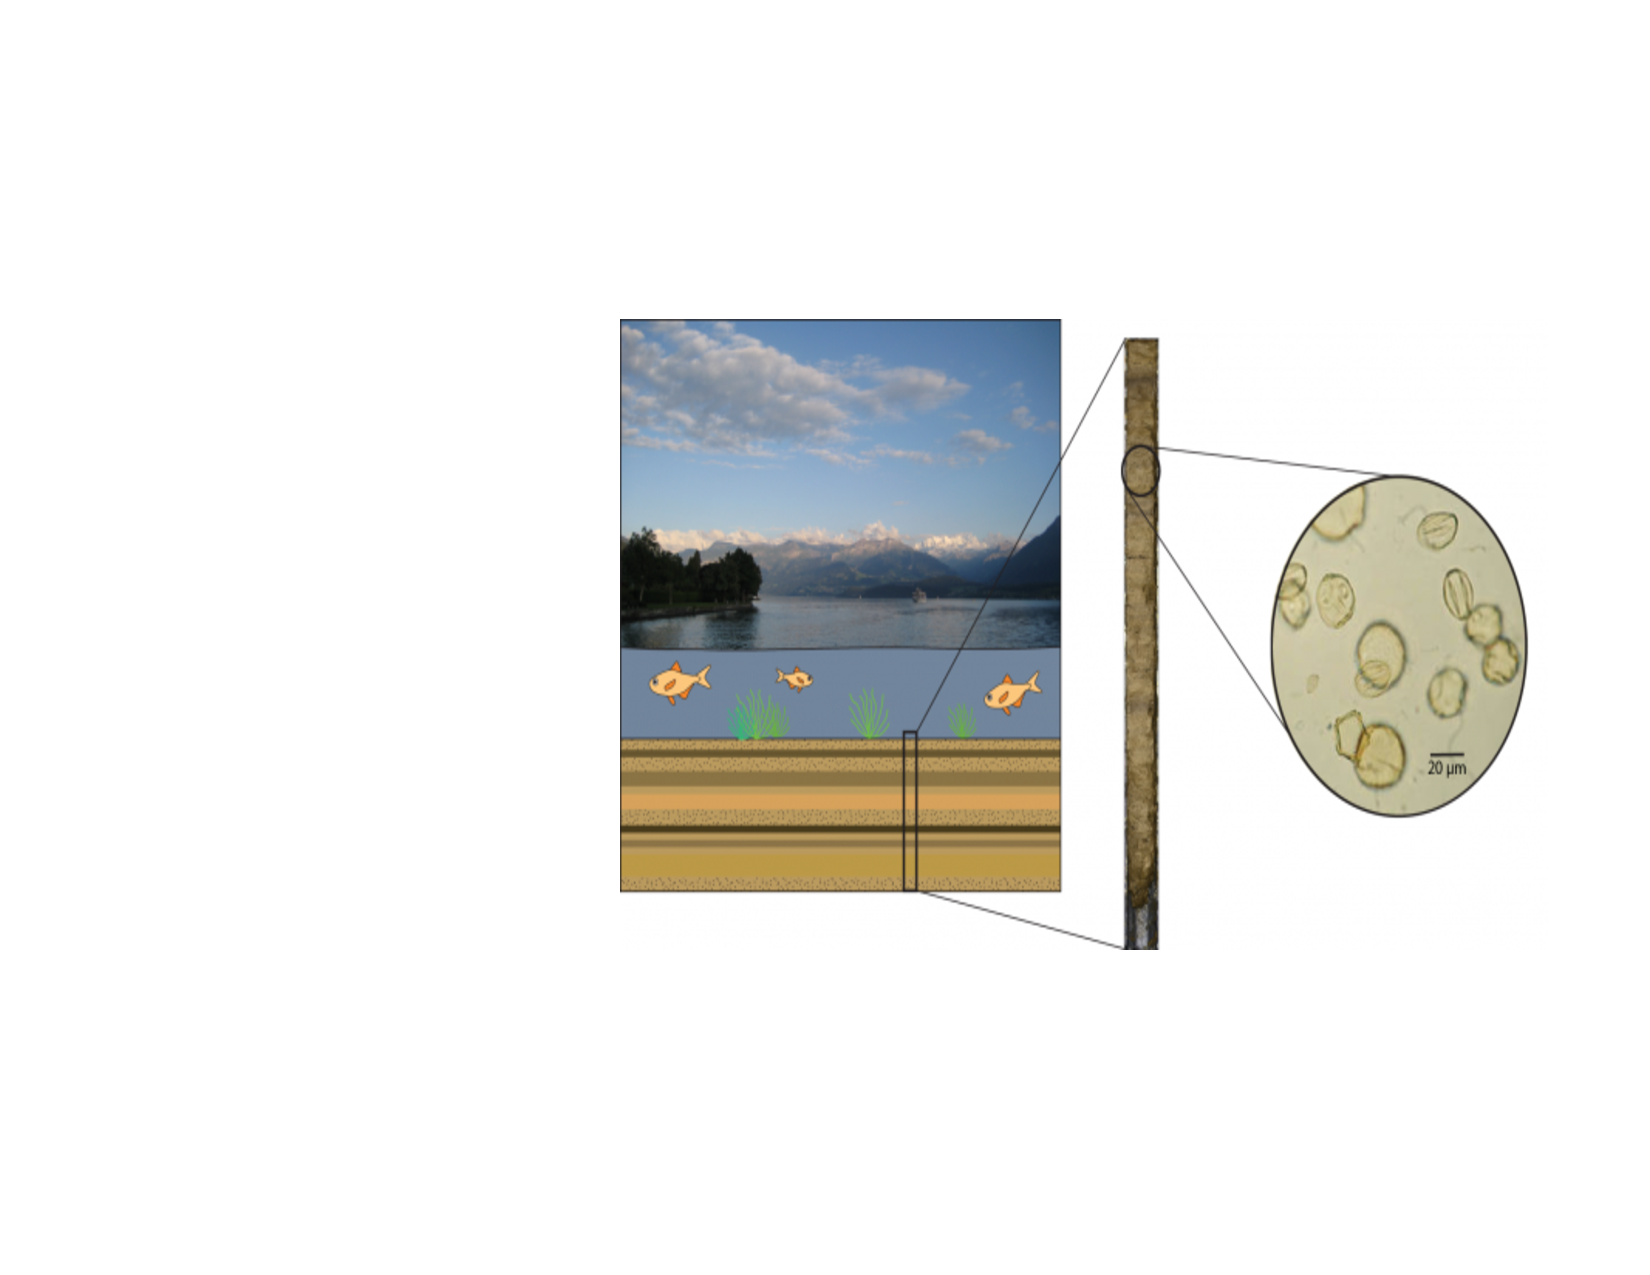
\includegraphics[width=.65\linewidth]{cores.pdf}
\end{figure}}

\only<3>
{\begin{figure}
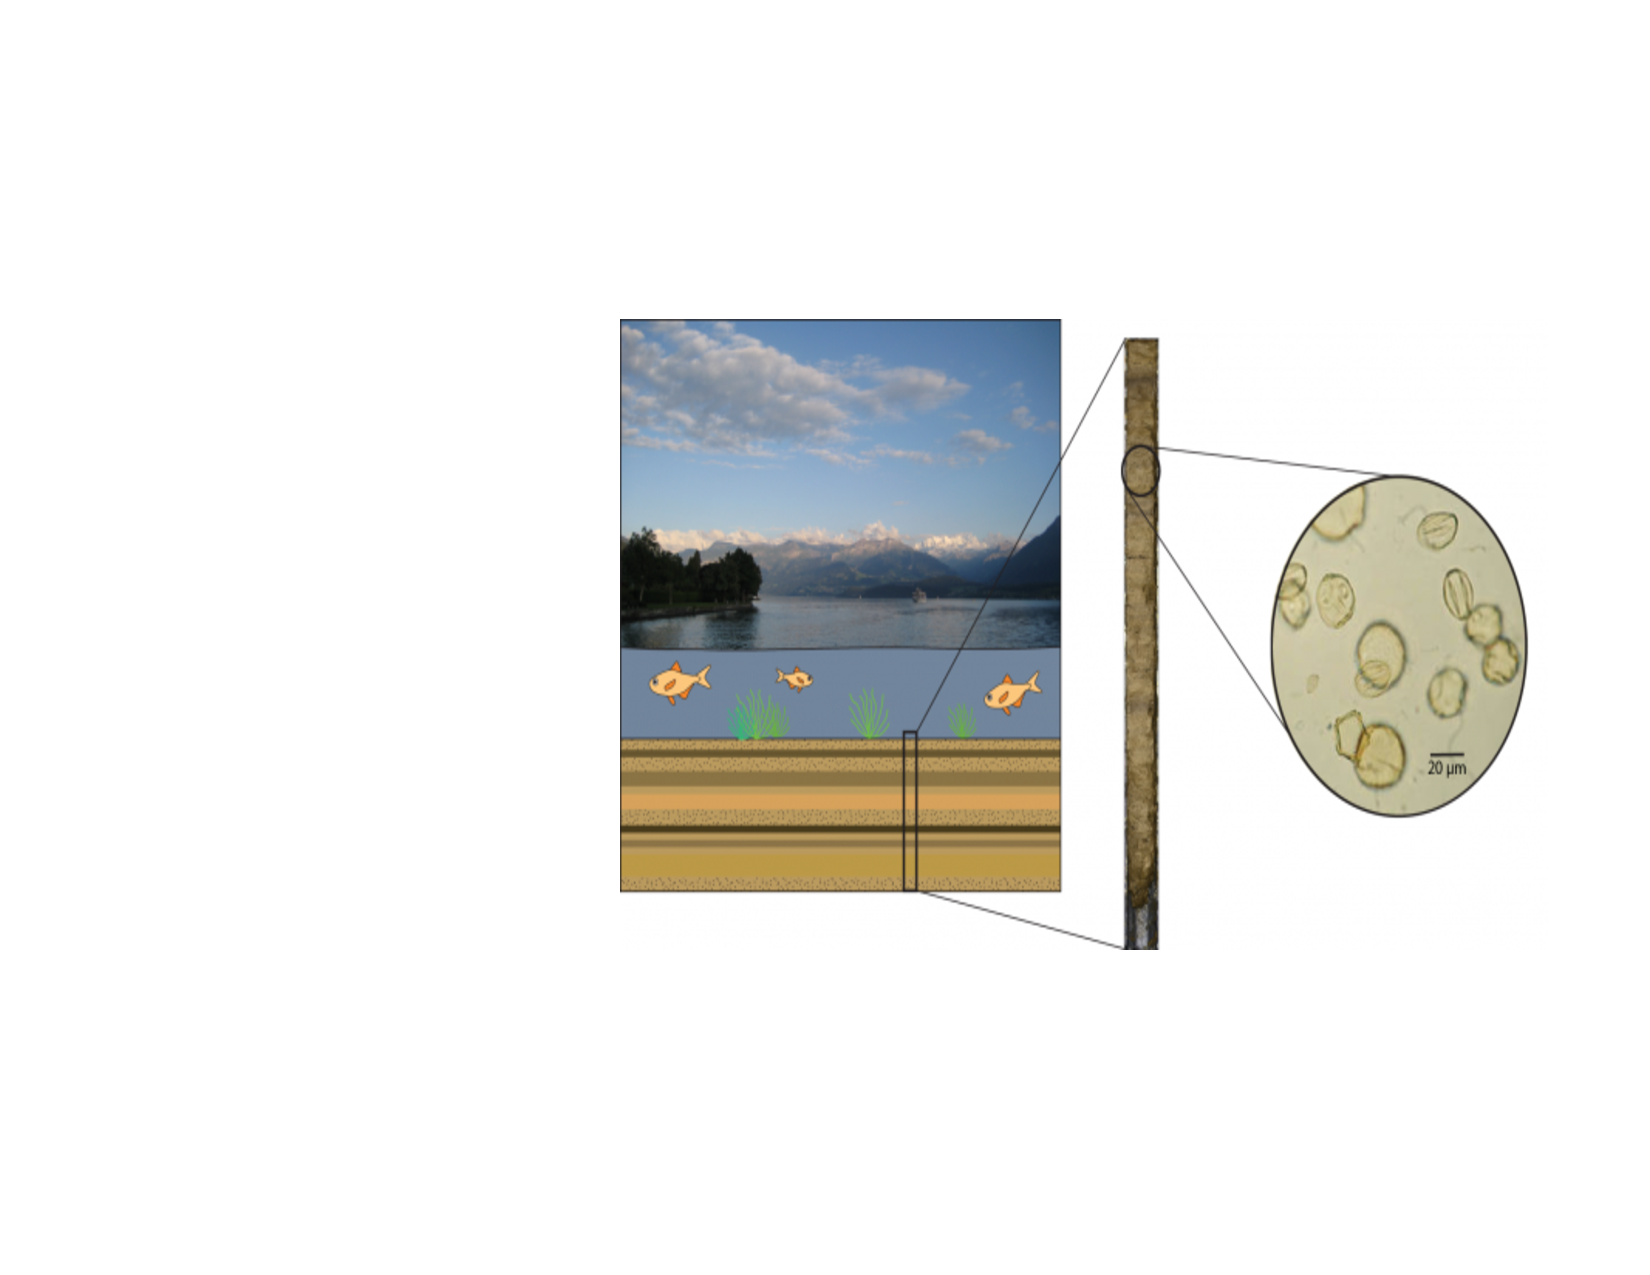
\includegraphics[width=.65\linewidth]{cores.pdf}
\end{figure}}
\end{frame}





%%%%%%%%%%%%%%%%%%%%%%%


\section{Current/ Future Work}


\begin{frame}

\frametitle{Future Work}
\only<1>{
\vspace{-.3in}
\begin{center}
\hspace*{-.3in}
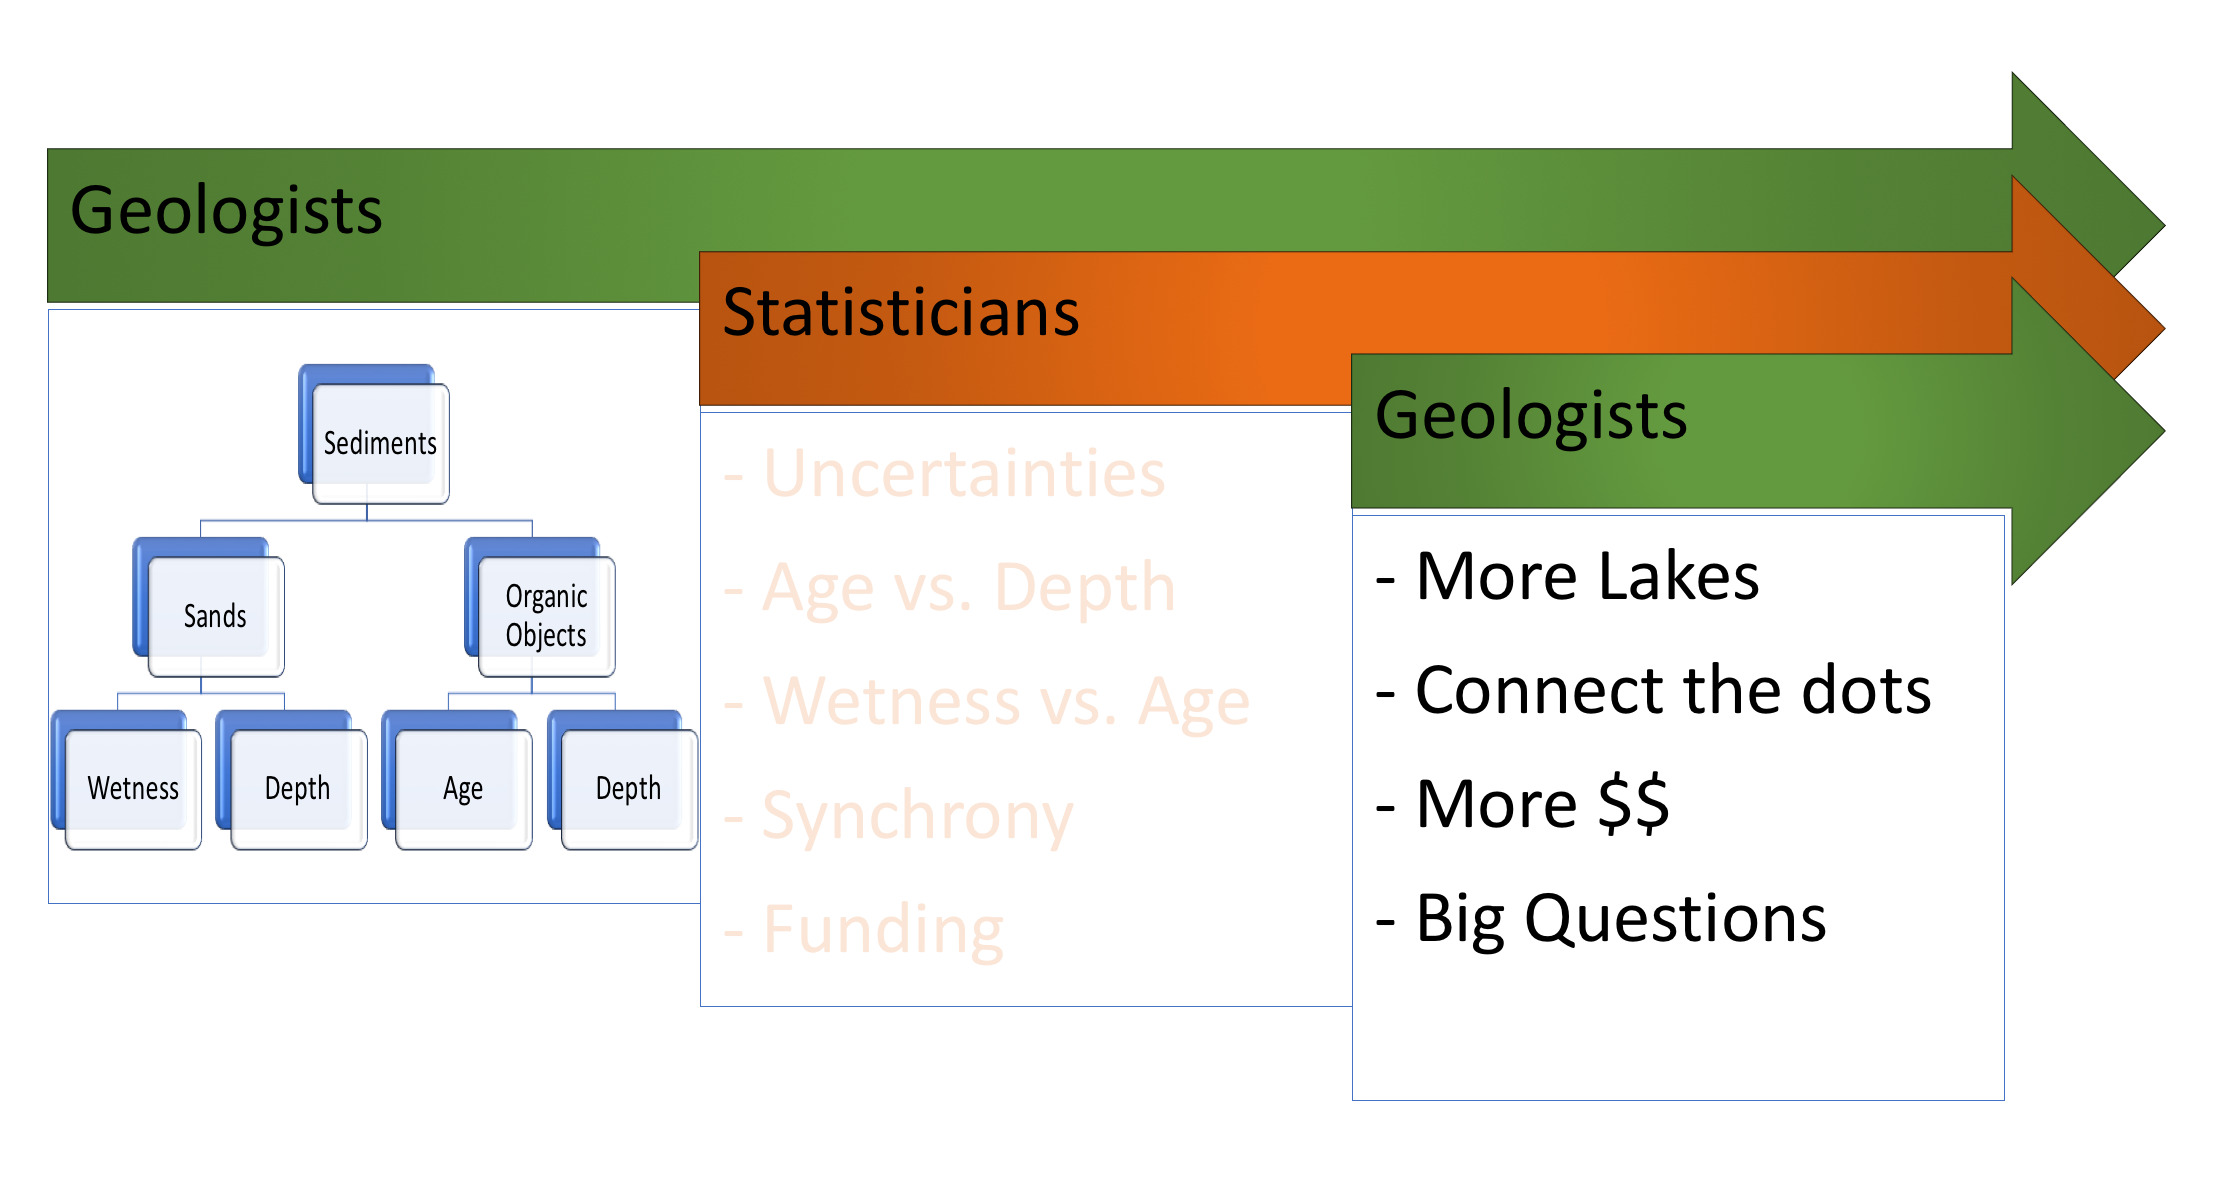
\includegraphics[width=1\textwidth]{page9}
\end{center}
}

\only<2>{
\vspace{-.3in}
\begin{center}
\hspace*{-.3in}
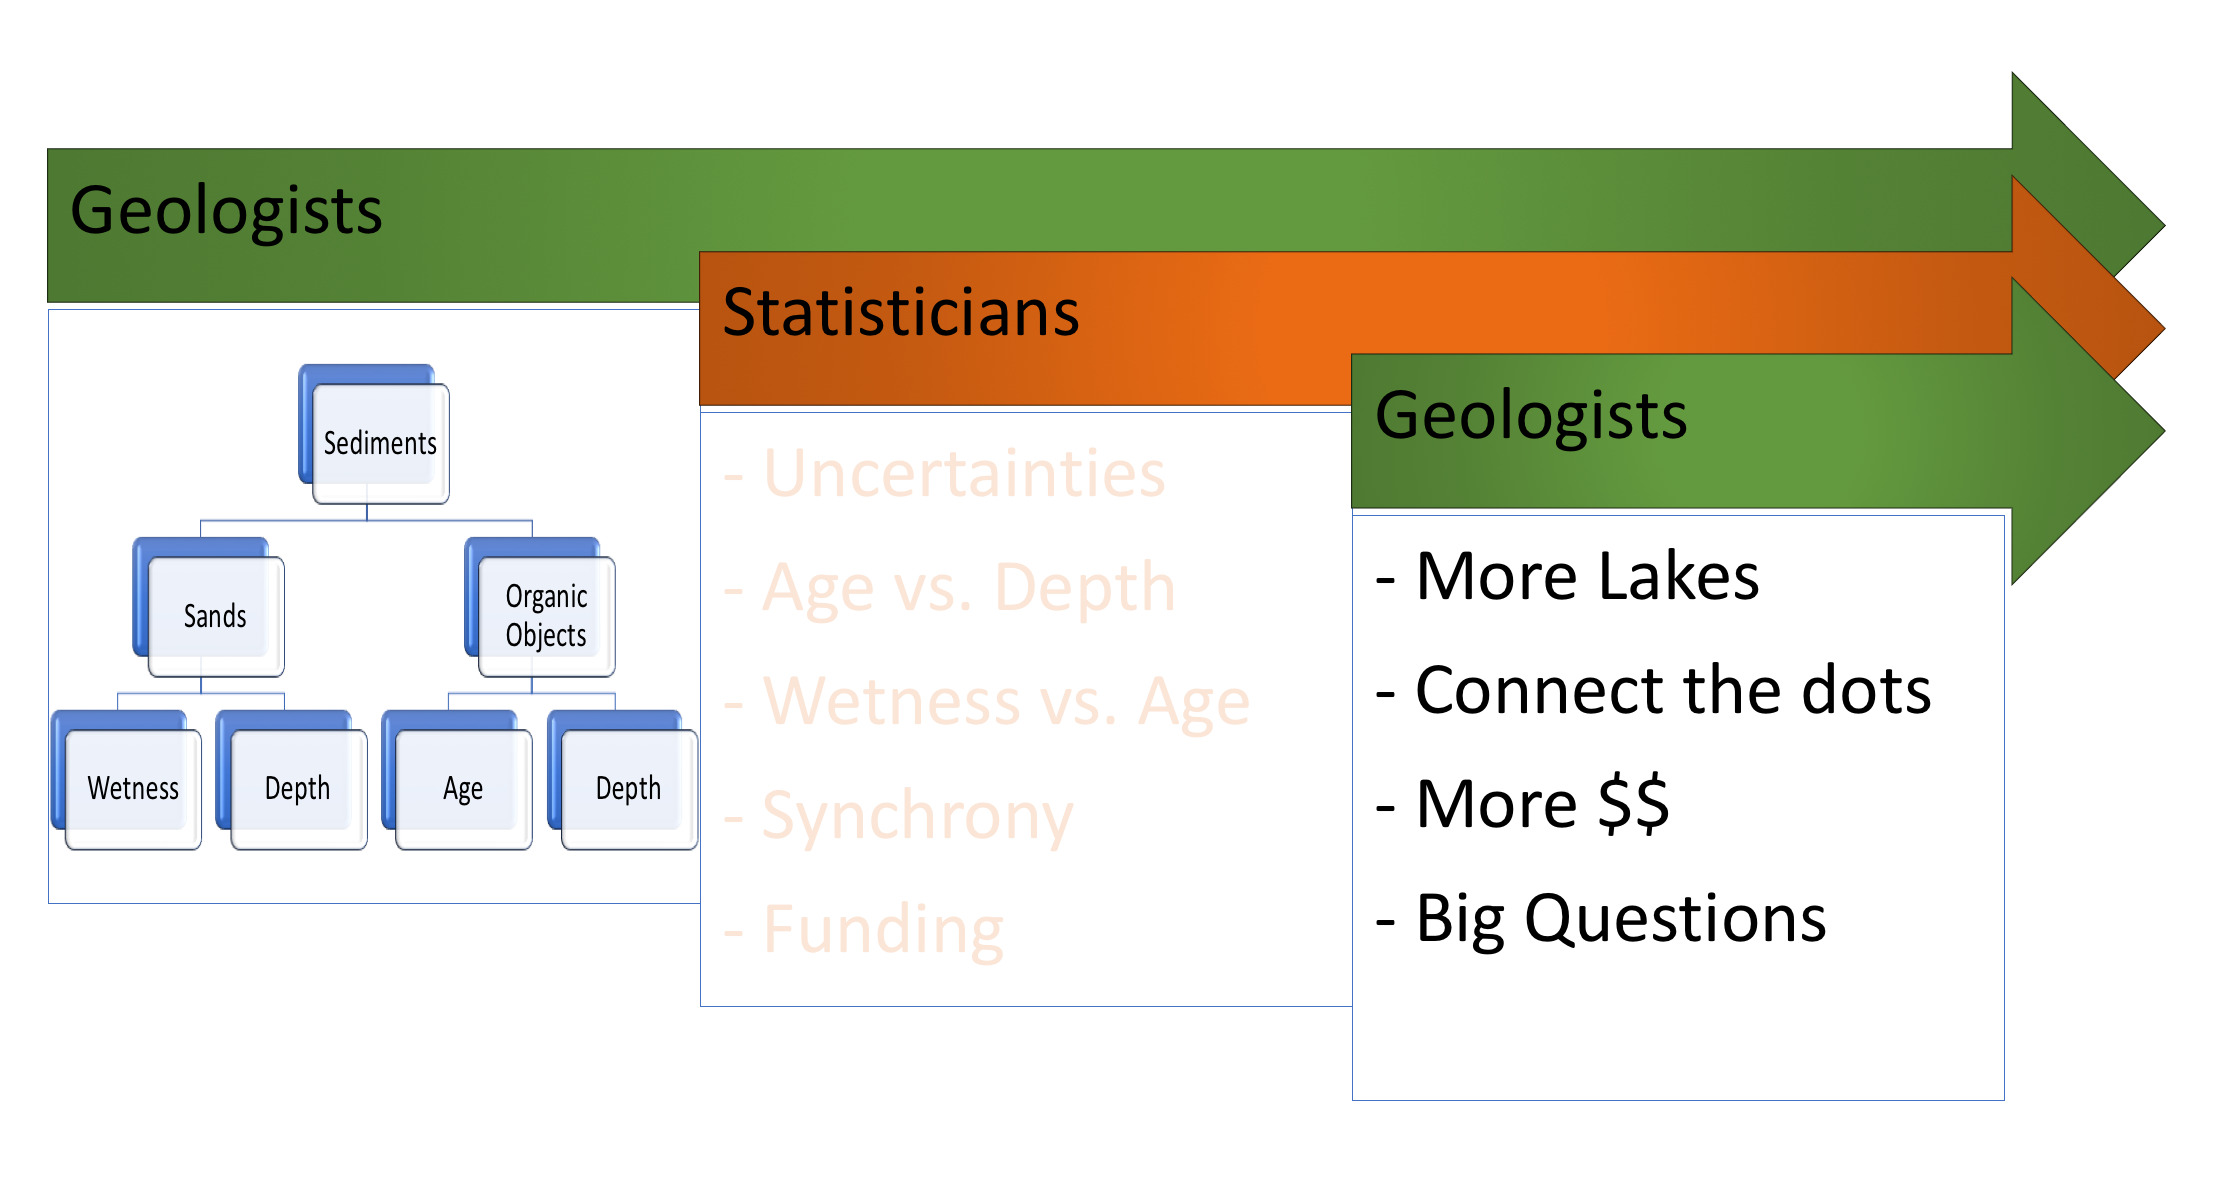
\includegraphics[width=1\textwidth]{page9}
\end{center}
}
\end{frame}


\section{Acknowledgments}
%\begin{frame}
%\frametitle{References}
%
%\begin{enumerate}
%%    \item Brooks, S. (2011). \emph{Handbook for Markov chain Monte Carlo}. Boca Raton: Taylor \& Francis.
%%    \vspace{-0.19cm}
%%    \item Givens, G. H., \& Hoeting, J. A. (2013). \emph{Computational statistics}. Oxford: Wiley-Blackwell.   
%%    \vspace{-0.19cm}
%%    \item Efron, B., \& Tibshirani, R. (1993). \emph{An introduction to the bootstrap}. New York: Chapman \& Hall.
%%\end{enumerate}
%
%\end{frame}
%



\begin{frame}
\frametitle{Acknowledgments}
\footnotesize{
\begin{thebibliography}{99} % Beamer does not support BibTeX so references must be inserted manually as below
%\bibitem[MAA, 2017]{p1} Mathematical Association of America Section (2017)
\bibitem[GRAM, 2016]{p1} Graduate Readiness and Access in Mathematics (Fall 2016)
\bibitem[Nichols, Kevin]{p2} Kevin Nichols  (Mentor)
\bibitem[Ramezan, Reza]{p3} Reza Ramezan (Mentor)
\bibitem[Kirby, Matthew]{p4} Matthew Kirby (Geologist Collaborator)
%\newblock Title of the publication
%\newblock \emph{Journal Name} 12(3), 45 -- 678.
\end{thebibliography}
}
\end{frame}

\begin{frame}
\begin{figure}
\begin{center}

\includegraphics[width=.7\textwidth]{pic1.png}
\end{center}
\end{figure}
\end{frame}

\end{document}




\begin{frame}
\frametitle{Bullet Points}
\begin{itemize}
\item Lorem ipsum dolor sit amet, consectetur adipiscing elit
\item Aliquam blandit faucibus nisi, sit amet dapibus enim tempus eu
\item Nulla commodo, erat quis gravida posuere, elit lacus lobortis est, quis porttitor odio mauris at libero
\item Nam cursus est eget velit posuere pellentesque
\item Vestibulum faucibus velit a augue condimentum quis convallis nulla gravida
\end{itemize}
\end{frame}

%------------------------------------------------


\begin{frame}
\frametitle{Blocks of Highlighted Text}
\begin{block}{Block 1}
Lorem ipsum dolor sit amet, consectetur adipiscing elit. Integer lectus nisl, ultricies in feugiat rutrum, porttitor sit amet augue. Aliquam ut tortor mauris. Sed volutpat ante purus, quis accumsan dolor.
\end{block}

\begin{block}{Block 2}
Pellentesque sed tellus purus. Class aptent taciti sociosqu ad litora torquent per conubia nostra, per inceptos himenaeos. Vestibulum quis magna at risus dictum tempor eu vitae velit.
\end{block}

\begin{block}{Block 3}
Suspendisse tincidunt sagittis gravida. Curabitur condimentum, enim sed venenatis rutrum, ipsum neque consectetur orci, sed blandit justo nisi ac lacus.
\end{block}
\end{frame}

%------------------------------------------------


\begin{frame}
\frametitle{Multiple Columns}
\begin{columns}[c] % The "c" option specifies centered vertical alignment while the "t" option is used for top vertical alignment

\column{.45\textwidth} % Left column and width
\textbf{Heading}
\begin{enumerate}
\item Statement
\item Explanation
\item Example
\end{enumerate}

\column{.5\textwidth} % Right column and width
Lorem ipsum dolor sit amet, consectetur adipiscing elit. Integer lectus nisl, ultricies in feugiat rutrum, porttitor sit amet augue. Aliquam ut tortor mauris. Sed volutpat ante purus, quis accumsan dolor.

\end{columns}
\end{frame}


\subsection{Tester}

\begin{frame}
\frametitle{Table}
\begin{table}
\begin{tabular}{l l l}
\toprule
\textbf{Treatments} & \textbf{Response 1} & \textbf{Response 2}\\
\midrule
Treatment 1 & 0.0003262 & 0.562 \\
Treatment 2 & 0.0015681 & 0.910 \\
Treatment 3 & 0.0009271 & 0.296 \\
\bottomrule
\end{tabular}
\caption{Table caption}
\end{table}
\end{frame}

%------------------------------------------------

\begin{frame}
\frametitle{Theorem}
\begin{theorem}[Mass--energy equivalence]
$E = mc^2$
\end{theorem}
\end{frame}

%------------------------------------------------

\begin{frame}[fragile] % Need to use the fragile option when verbatim is used in the slide
\frametitle{Verbatim}
\begin{example}[Theorem Slide Code]
\begin{verbatim}
\begin{frame}
\frametitle{Theorem}
\begin{theorem}[Mass--energy equivalence]
$E = mc^2$
\end{theorem}
\end{frame}\end{verbatim}
\end{example}
\end{frame}

%------------------------------------------------

\begin{frame}
\frametitle{Figure}
Uncomment the code on this slide to include your own image from the same directory as the template .TeX file.
\begin{figure}
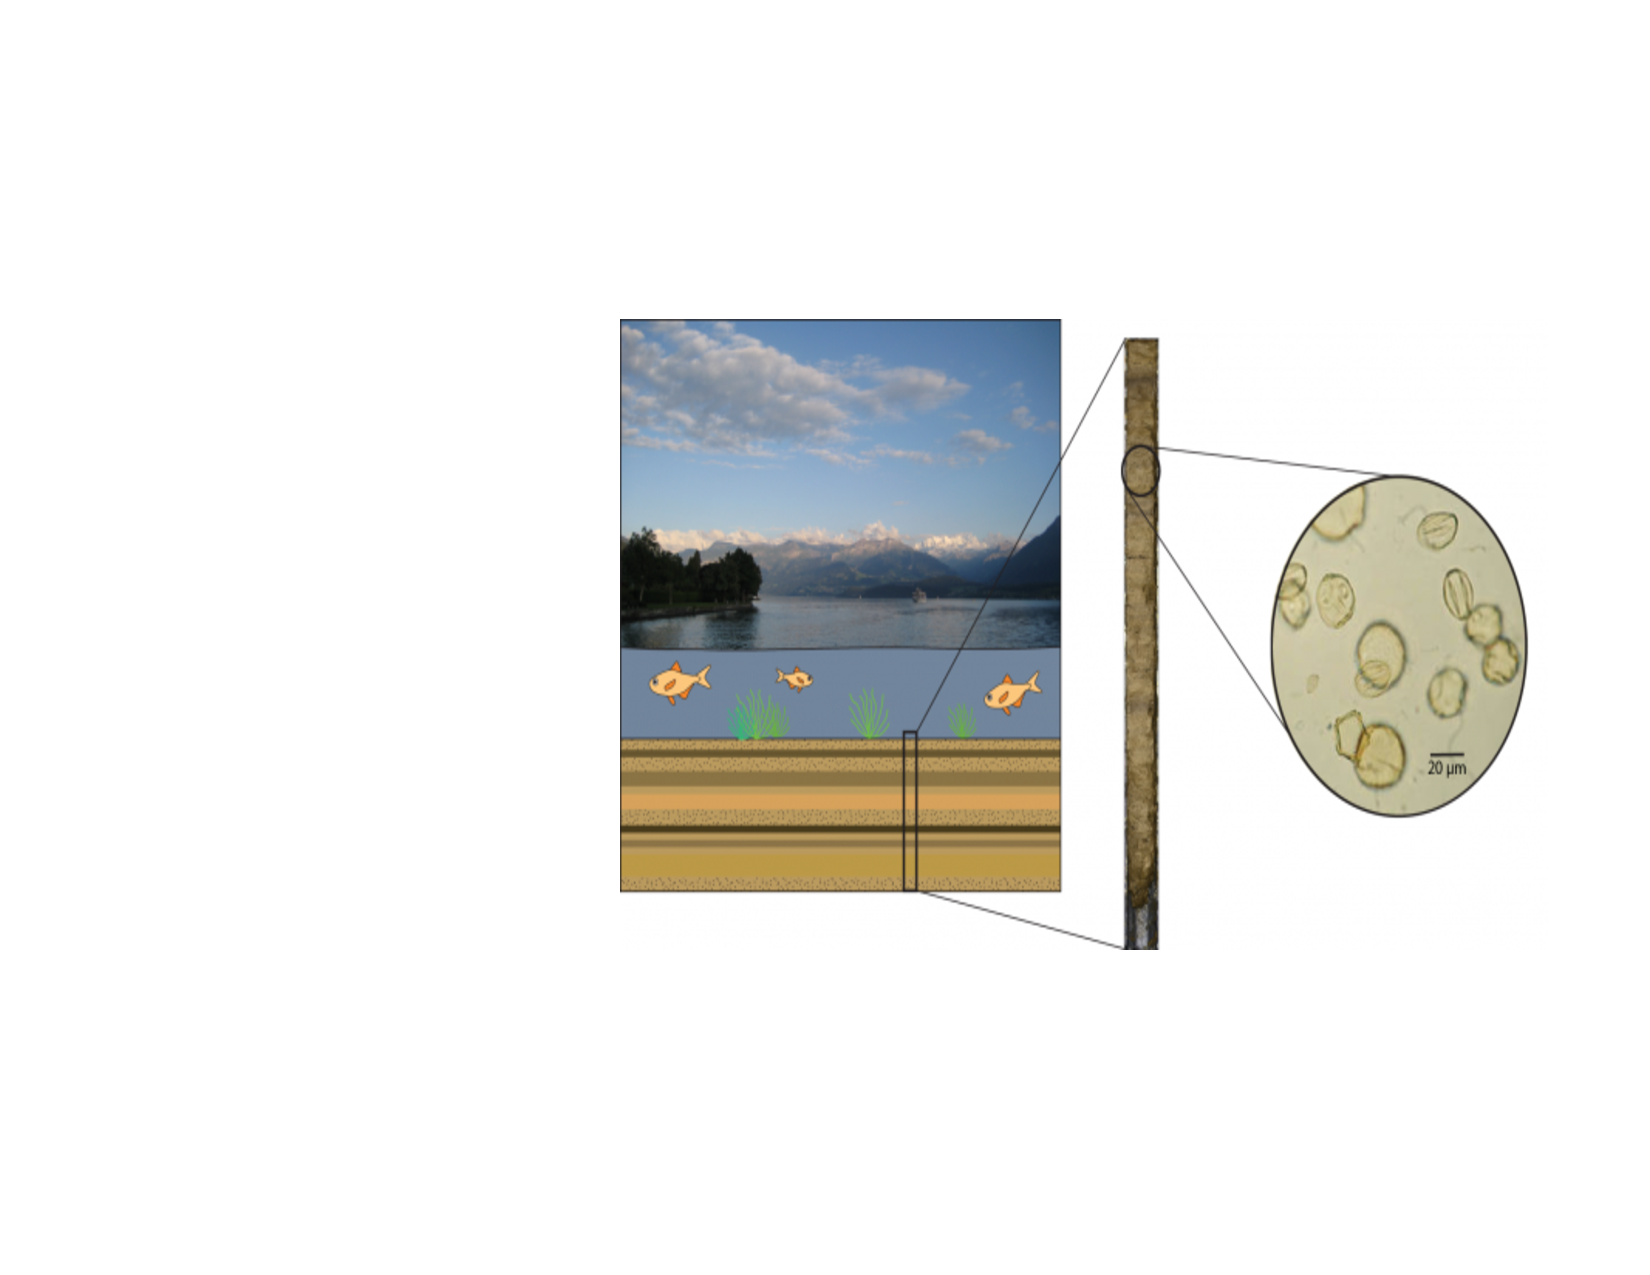
\includegraphics[width=0.8\linewidth]{cores.pdf}
\end{figure}
\end{frame}

%------------------------------------------------

\begin{frame}[fragile] % Need to use the fragile option when verbatim is used in the slide
\frametitle{Citation}
An example of the \verb|\cite| command to cite within the presentation:\\~

This statement requires citation \cite{p1}.
\end{frame}

%------------------------------------------------


%------------------------------------------------

\begin{frame}
\Huge{\centerline{The End}}
\end{frame}

%----------------------------------------------------------------------------------------

 